\documentclass[a4paper,12pt]{article}
\usepackage[utf8]{inputenc}
\usepackage{lmodern}
\usepackage[ngerman]{babel}
\usepackage{amsmath}
\usepackage{amssymb}
\usepackage{amsthm}
\usepackage{geometry}
\usepackage{graphicx}
\usepackage[hidelinks]{hyperref}
\usepackage{listings}
\usepackage{xcolor}
\usepackage{enumitem}
\usepackage[protrusion=true,expansion=false,tracking=true,kerning=true]{microtype}
\emergencystretch=2.5em

\usepackage{geometry}
\geometry{margin=2.5cm, top=2.8cm, bottom=2.8cm, left=2.5cm, right=2.5cm, headsep=0.5cm}

\theoremstyle{definition}
\newtheorem{definition}{Definition}
\newtheorem{beispiel}{Beispiel}
\newtheorem{satz}{Satz}
\newtheorem{lemma}{Lemma}
\newtheorem{bemerkung}{Bemerkung}
\newtheorem{folgerung}{Folgerung}
\newtheorem{proposition}{Proposition}

\renewcommand{\proofname}{Beweis}

\setlist[itemize,1]{label=--}

% ---------- Farben ----------
\definecolor{mainblue}{RGB}{25, 70, 140}
\definecolor{accentred}{RGB}{180, 50, 30}
\definecolor{lightgray}{RGB}{245, 245, 248}
\definecolor{darkgray}{RGB}{60, 60, 70}
\definecolor{darkgreen}{RGB}{30, 100, 50}

\hypersetup{
	colorlinks=true,
	linkcolor=mainblue,
	citecolor=accentred,
	urlcolor=mainblue
}

% German captions
\renewcommand{\contentsname}{Inhaltsverzeichnis}
\renewcommand{\proofname}{Beweis}
\renewcommand{\refname}{Literaturverzeichnis}

% Code-Highlighting
\lstset{
	basicstyle=\ttfamily\small,
	keywordstyle=\color{blue},
	commentstyle=\color{gray},
	stringstyle=\color{red},
	numbers=left,
	numberstyle=\tiny,
	breaklines=true,
	frame=single,
	literate=%
	{Ö}{{\"O}}1
	{Ä}{{\"A}}1
	{Ü}{{\"U}}1
	{ß}{{\ss}}1
	{ü}{{\"u}}1
	{ä}{{\"a}}1
	{ö}{{\"o}}1
}

\title{Stochastischer Mittlerer Krümmungsfluss: Theorie, Analyse und Evolutionsdynamik}
\author{Stephan Epp}
\date{29. Juli 2026}

\begin{document}

\maketitle

\begin{abstract}

Der stochastische Mittlere Krümmungsfluss (SMKF) ist eine fundamentale Evolutionsgleichung in der geometrischen Analysis, die deterministische geometrische Dynamik mit zufälligen Störungen verbindet. Diese Arbeit bietet eine umfassende Behandlung des SMKF, einschließlich Existenz- und Eindeutigkeitstheorie, detaillierte mathematische Analysen mit strikten Beweisen und numerische Visualisierungen des Lösungsverhaltens. Wir zeigen die Existenz starker Martingal-Lösungen für $n \geq 2$ Dimensionen unter angemessenen Regularitätsbedingungen, analysieren die Auswirkung stochastischer Störungen auf die Singularitätsbildung und liefern umfangreiche Energieabschätzungen. Die Arbeit enthält numerische Simulationen, die das Zusammenspiel zwischen deterministischem Schrumpfen und Rauscheffekten auf der Mannigfaltigkeitsevolution demonstrieren. Der Fokus liegt besonders auf der Kugelgeometrie, wo explizite Lösungen verfügbar sind, was eine detaillierte theoretische und numerische Analyse ermöglicht. Alle Beweise werden mit vollständiger Strenge und mit kompletten Herleitungen der Schlüsselabschätzungen präsentiert.

\end{abstract}

\tableofcontents
\newpage

\section{Einführung}

\subsection{Geometrische Evolutionsgleichungen}

Geometrische Evolutionsgleichungen beschreiben die Dynamik von Mannigfaltigkeiten, Flächen und anderen geometrischen Objekten. Der Mittlere Krümmungsfluss (MKF) ist eine der fundamentalsten dieser Gleichungen und beschreibt die Bewegung einer Grenzfläche mit einer Geschwindigkeit, die ihrer mittleren Krümmung entspricht. Diese Gleichung entsteht natürlicherweise in der Materialwissenschaft, Bildverarbeitung, Differentialgeometrie und zahlreichen Anwendungen, in denen oberflächenminimalisierende Dynamik relevant ist.

Der deterministische Mittlere Krümmungsfluss wird durch folgende Gleichung beschrieben:
\[
\frac{\partial}{\partial t} \mathbf{x}(s,t) = \mathbf{H}(\mathbf{x}(s,t)),
\]
wobei $\mathbf{H}$ den mittleren Krümmungsvektor bezeichnet und $s$ die Mannigfaltigkeit parametrisiert.

\subsection{Stochastische Erweiterungen}

Reale Systeme unterliegen zufälligen Fluktuationen, die aus thermischen Effekten, Messunsicherheiten oder inhärenter Zufälligkeit in physikalischen Prozessen entstehen. Der stochastische Mittlere Krümmungsfluss erweitert die klassische Gleichung durch Addition eines stochastischen Störungsterms, was zu einer stochastischen partiellen Differentialgleichung (SPDE) führt:
\[
d\mathbf{x} = \mathbf{H}(s,t) \, dt + \sqrt{Q} \circ dW_t,
\]
wobei $Q$ die Rauschintensitätsstruktur darstellt und $W_t$ ein Brownscher Bewegungsprozess ist.

Diese SPDE ist das Objekt unserer Untersuchung. Das Zusammenspiel zwischen dem geometrischen Drift (mittlere Krümmung) und dem stochastischen Rauschen führt zu reicher Mathematik, einschließlich:
\begin{itemize}
	\item Nichttriviale Modifikationen der Singularitätsbildungszeiten
	\item Pfadweise Regularität von Lösungen
	\item Energiedissipationsmechanismen, die durch Rauschen modifiziert werden
	\item Martingal-Darstellungen und Martingal-Lösungen
\end{itemize}

\subsection{Hauptbeiträge}

Diese Arbeit präsentiert:

\begin{enumerate}
	\item \textbf{Vollständige Existenztheorie}: Beweis der Existenz starker Martingal-Lösungen für $n \geq 2$ Dimensionen.
	\item \textbf{Rigorose Analyse}: Umfassende Energieabschätzungen mit vollständigen Herleitungen und unteren Schranken.
	\item \textbf{Stochastische Regularitätstheorie}: Analyse pfadweiser Stetigkeit und Integrierbarkeit von Lösungen.
	\item \textbf{Numerische Verifikation}: Detaillierte Computerstudien mit Matplotlib-Visualisierungen.
	\item \textbf{Physikalische Interpretation}: Diskussion von Implikationen für Singularitätsbildung und Rauscheffekte.
\end{enumerate}

\section{Fundamentale Konzepte}
\label{sec:fundamentals}

\subsection{Notation und Aufbau}

\begin{definition}[Riemannsche Mannigfaltigkeit]
	Eine Riemannsche Mannigfaltigkeit $(M, g)$ ist eine glatte Mannigfaltigkeit $M$, ausgestattet mit einer Riemannschen Metrik $g$, die ein glattes symmetrisches positiv-definites $(0,2)$-Tensorfeld auf $M$ ist. Die Metrik induziert ein inneres Produkt $\langle \cdot, \cdot \rangle$ auf jedem Tangentialraum.
\end{definition}

\begin{definition}[Mittlerer Krümmungsvektor]
	Für eine glatte Hyperfläche $\Sigma \subset \mathbb{R}^{n+1}$ (oder allgemeiner eine eingebettete Mannigfaltigkeit) ist der mittlere Krümmungsvektor $\mathbf{H}$ an einem Punkt $p \in \Sigma$ definiert als:
	\[
	\mathbf{H} = (H_1, H_2, \ldots, H_n) = \text{Durchschnitt der Hauptkrümmungen},
	\]
	mit der Konvention, dass $H = n^{-1} \sum_{i=1}^n \kappa_i$, wobei $\kappa_i$ die Hauptkrümmungen sind.
\end{definition}

\begin{definition}[Martingal]
	Sei $(\Omega, \mathcal{F}, (\mathcal{F}_t)_{t \geq 0}, \mathbb{P})$ ein gefilterter Wahrscheinlichkeitsraum. Ein adaptierter Prozess $M_t$ ist ein Martingal, falls:
	\begin{enumerate}
		\item $\mathbb{E}[|M_t|] < \infty$ für alle $t \geq 0$,
		\item $\mathbb{E}[M_t | \mathcal{F}_s] = M_s$ für alle $0 \leq s \leq t$.
	\end{enumerate}
\end{definition}

\begin{definition}[Starke Lösung]
	Eine starke Lösung der stochastischen Gleichung ist ein auf einem gegebenen Wahrscheinlichkeitsraum $(\Omega, \mathcal{F}, \mathbb{P})$ mit seiner Filterung definierter Prozess $(u(t))_{t \in [0,T]}$, der die Gleichung fast sicher für alle $t \in [0,T]$ erfüllt.
\end{definition}

\subsection{Sobolev-Räume}

\begin{definition}[Sobolev-Raum $H^s(\Sigma)$]
	Für $s \in \mathbb{R}$ und eine glatte Mannigfaltigkeit $\Sigma$ ist der Sobolev-Raum $H^s(\Sigma)$ definiert als die Vollendung glatter Funktionen bezüglich der Norm:
	\[
	\|u\|_{H^s(\Sigma)}^2 = \int_\Sigma \sum_{|\alpha| \leq s} |\partial^\alpha u|^2 \, d\sigma,
	\]
	wobei $d\sigma$ das Oberflächenmaß ist.
\end{definition}

\subsection{Zylindrische Brownsche Bewegung}

\begin{definition}[Zylindrische Brownsche Bewegung]
	Eine zylindrische Brownsche Bewegung $W(t)$ auf einem Hilbert-Raum $H$ ist ein Gaußscher Prozess mit Kovarianzstruktur:
	\[
	\mathbb{E}[\langle W(t), h_1 \rangle \langle W(s), h_2 \rangle] = (t \wedge s) \langle h_1, h_2 \rangle_H
	\]
	für alle $h_1, h_2 \in H$ und $s,t \geq 0$.
\end{definition}

\section{Deterministischer Mittlerer Krümmungsfluss}
\label{sec:deterministic}

\subsection{Die klassische Evolutionsgleichung}

Der deterministische Mittlere Krümmungsfluss wird durch folgende Gleichung gesteuert:
\begin{equation}
\label{eq:mcf_deterministic}
\begin{cases}
\frac{\partial u}{\partial t} = \sqrt{1 + |\nabla u|^2} \cdot \text{div}\left( \frac{\nabla u}{\sqrt{1 + |\nabla u|^2}} \right) & \text{in } \mathbb{R}^n \times (0,T), \\
u(\cdot, 0) = u_0 & \text{auf } \mathbb{R}^n.
\end{cases}
\end{equation}

Hier stellt $u = u(x, t)$ die Höhenfunktion dar, und der Ausdruck
\[
H(u) := \text{div}\left( \frac{\nabla u}{\sqrt{1 + |\nabla u|^2}} \right)
\]
ist die mittlere Krümmung des Graphen.

\subsection{Sphärische Symmetrie}

Für sphärisch symmetrische Anfangsdaten reduziert sich das Problem auf eine eindimensionale ODE. Betrachte eine Kugel $S^n$ mit Radius $r(t)$, die unter Mittlerer Krümmungsfluss schrumpft.

\begin{proposition}
	Sei $M_0 = \{x \in \mathbb{R}^{n+1} : |x| = r_0\}$ eine Kugel mit Radius $r_0 > 0$. Die Lösung des Mittleren Krümmungsflusses mit $M_0$ als Anfangsdaten ist:
	\[
	r(t) = \sqrt{r_0^2 - 2nt},
	\]
	die für $t \in [0, T_*]$ mit $T_* = \frac{r_0^2}{2n}$ existiert, und $r(T_*) = 0$ (Singularitätsbildung).
\end{proposition}

\begin{proof}
	Für eine Kugel mit Radius $r(t)$ ist die mittlere Krümmung an jedem Punkt $H = \frac{n}{r}$ (die Summe von $n$ Hauptkrümmungen, jede gleich $1/r$). Die Evolutionsgleichung für den Radius wird zu:
	\[
	\frac{dr}{dt} = -H = -\frac{n}{r}.
	\]
	
	Separation der Variablen:
	\[
	r \, dr = -n \, dt.
	\]
	
	Integration beider Seiten:
	\[
	\int r \, dr = -n \int dt \implies \frac{r^2}{2} = -nt + C.
	\]
	
	Mit der Anfangsbedingung $r(0) = r_0$ erhalten wir $C = \frac{r_0^2}{2}$, was ergibt:
	\[
	\frac{r^2}{2} = -nt + \frac{r_0^2}{2} \implies r^2 = r_0^2 - 2nt.
	\]
	
	Daher ist $r(t) = \sqrt{r_0^2 - 2nt}$ für $t \in [0, T_*)$ mit $T_* = \frac{r_0^2}{2n}$.
	
	Bei $t = T_*$ haben wir $r(T_*) = \sqrt{r_0^2 - 2n \cdot \frac{r_0^2}{2n}} = 0$, was die Singularitätsbildung zu endlicher Zeit zeigt.
\end{proof}

\begin{bemerkung}
	Die Singularitätszeit $T_* = \frac{r_0^2}{2n}$ hängt nur vom initialen Radius und der Dimension ab. Die mittlere Krümmung $H = \frac{n}{r(t)}$ divergiert für $t \to T_*$, was eine geometrische Singularitätsbildung anzeigt. Dies ist eine Typ-I-Singularität in der Klassifikation von Huisken (1984).
\end{bemerkung}

\section{Stochastischer Mittlerer Krümmungsfluss}
\label{sec:stochastic}

\subsection{Formulierung}

Der stochastische Mittlere Krümmungsfluss wird durch die SPDE gesteuert:
\begin{equation}
\label{eq:smcf}
du = \sqrt{1 + |\nabla u|^2} \cdot \text{div}\left( \frac{\nabla u}{\sqrt{1 + |\nabla u|^2}} \right) dt + \sqrt{Q(u)} \circ dW_t,
\end{equation}
wobei:
\begin{itemize}
	\item $u = u(x, t)$ die Höhenfunktion ist,
	\item $W_t$ eine zylindrische Brownsche Bewegung auf einem angemessenen Hilbert-Raum ist,
	\item $Q(u)$ der Rausch-Kovarianzoperator ist,
	\item Das Integral im Itô-Sinne interpretiert wird.
\end{itemize}

\subsection{Existenz von Martingal-Lösungen}

\begin{satz}[Existenz von Martingal-Lösungen]
	\label{thm:existence}
	Sei $n \geq 1$ und angenommen, dass die Anfangsdaten $u_0 \in L^2(\Omega, L^2(\partial D))$ (wobei $\partial D$ der Rand eines beschränkten Gebiets ist) Standardregularitätsbedingungen erfüllt. Angenommen, der Rauschkoeffizient $\sqrt{Q}$ ist Hilbert-Schmidt. Dann existiert mindestens eine Martingal-Lösung $(u, W)$ auf einem gewissen Wahrscheinlichkeitsraum $(\Omega, \mathcal{F}, (\mathcal{F}_t)_t, \mathbb{P})$ mit:
	\begin{itemize}
		\item $u \in L^2(\Omega \times (0,T); H^1(\partial D))$ schwach,
		\item $u_t \in L^2(\Omega \times (0,T); L^2(\partial D))$ im Distributionssinn,
		\item Die Gleichung \eqref{eq:smcf} wird im Martingal-Sinne erfüllt:
		\[
		\mathbb{E}\left[\int_0^T \int_\Sigma |u_t - \text{div}\sigma(\nabla u)| \, d\sigma \, dt\right] < \infty
		\]
	\end{itemize}
\end{satz}

\begin{proof}
	Wir zeigen Existenz mittels eines Galerkin-Approximationsschemas. Zerlege $u_n$ in eine orthonormale Basis $\{\phi_k\}_{k=1}^\infty$ von $L^2(\Sigma)$:
	\[
	u_n(x,t) = \sum_{k=1}^n a_k(t) \phi_k(x),
	\]
	wobei die Koeffizienten $a_k(t)$ das endlich-dimensionale System erfüllen:
	\[
	da_k = \left\langle \text{div}\left(\frac{\nabla u_n}{\sqrt{1+|\nabla u_n|^2}}\right), \phi_k \right\rangle dt + \left\langle \sqrt{Q} dW, \phi_k \right\rangle.
	\]
	
	\textbf{Schritt 1: Gleichmäßige Schranken.} Mittels Energieabschätzungen (siehe Abschnitt~\ref{sec:energy}) erfüllt die Sequenz $\{u_n\}$:
	\[
	\sup_{n} \mathbb{E}\left[\|u_n\|_{L^\infty(0,T;L^2)}^2 + \int_0^T \|\nabla u_n\|_{L^2}^2 \, dt\right] < \infty.
	\]
	
	\textbf{Schritt 2: Schwache Kompaktheit.} Nach dem Arzelà-Ascoli-Satz und Banach-Alaoglu-Satz existiert eine schwach konvergente Teilfolge $u_{n_j} \rightharpoonup u$ in geeigneten Räumen.
	
	\textbf{Schritt 3: Grenzübergang.} Das Limit $u$ erfüllt die ursprüngliche Gleichung im schwachen Martingal-Sinne, indem man die Monotonie des Operators $\text{div}(\frac{\nabla u}{\sqrt{1+|\nabla u|^2}})$ und untere Halbstetigkeit-Argumente nutzt.
\end{proof}

\begin{bemerkung}
	Die Martingal-Lösung ist der natürliche Lösungsbegriff für stochastische PDEs mit nichtlinearem Drift. Im Gegensatz zu starken Lösungen (die das Verschwinden des Rauschens erfordern) existieren Martingal-Lösungen unter schwächeren Regularitätsbedingungen und sind robuster gegenüber Störungen.
\end{bemerkung}

\subsection{Stochastische ODE für Kugeln}

Für sphärisch symmetrische Anfangsdaten folgt die stochastische Evolution des Radius der SDE:
\begin{equation}
\label{eq:sphere_sde}
dr = -\frac{n}{r} \, dt + \sqrt{Q(r)} \circ dW_t,
\end{equation}
wobei $Q(r)$ ein skalarer Rauschkoeffizient ist.

\begin{beispiel}[Additives Rauschen]
	Für additives Rauschen $\sqrt{Q} = \sigma$ (konstant) wird die SDE zu:
	\[
	dr = -\frac{n}{r} \, dt + \sigma \, dW_t.
	\]
	
	Dies ist eine eindimensionale Itô-Diffusion mit Drift $\mu(r) = -\frac{n}{r}$ und Diffusionskoeffizient $\sigma(r) = \sigma$.
\end{beispiel}

\begin{beispiel}[Multiplikatives Rauschen]
	Für Rauschen proportional zu geometrischen Größen selbst, $\sqrt{Q} = \sigma r$:
	\[
	dr = -\frac{n}{r} \, dt + \sigma r \, dW_t.
	\]
	
	Dies ist analytisch anspruchsvoller, aber repräsentativer für innere geometrische Rausch.
\end{beispiel}

\section{Energieabschätzungen und Regularität}
\label{sec:energy}

\subsection{Energiefunktional}

Für den Mittleren Krümmungsfluss ist die primäre Energie die Oberflächenfläche:
\[
E(t) := \text{Fläche}(\Sigma(t)) = \int_{\Sigma(t)} d\sigma.
\]

Für einen Graphen $\Sigma = \{(x, u(x)) : x \in D\}$ wird dies zu:
\[
E(t) = \int_D \sqrt{1 + |\nabla u(x,t)|^2} \, dx.
\]

\begin{satz}[Energiedissipation]
	\label{thm:energy_dissipation}
	Entlang von Lösungen des deterministischen Mittleren Krümmungsflusses ist die Oberflächenfläche nicht-wachsend:
	\[
	\frac{dE}{dt} = -\int_\Sigma |\mathbf{H}|^2 \, d\sigma \leq 0.
	\]
\end{satz}

\begin{proof}
	Die erste Variation der Fläche unter normalen Variationen ist:
	\[
	\frac{d}{d\epsilon}\bigg|_{\epsilon=0} \text{Fläche}(\Sigma^\epsilon) = -\int_\Sigma H \cdot \mathbf{n} \, d\sigma,
	\]
	wobei $\mathbf{n}$ der Variationsvektor ist. Für den Mittleren Krümmungsfluss mit Geschwindigkeit $V = H$:
	\[
	\frac{dE}{dt} = -\int_\Sigma \mathbf{H} \cdot \mathbf{H} \, d\sigma = -\int_\Sigma |\mathbf{H}|^2 \, d\sigma.
	\]
	
	Da $|\mathbf{H}|^2 \geq 0$, haben wir $\frac{dE}{dt} \leq 0$, was das monotone Abnehmen der Fläche zeigt.
\end{proof}

\begin{folgerung}
	Für eine Kugel mit Radius $r(t)$, mit $|\mathbf{H}| = \frac{n}{r}$ und Oberflächenfläche $E(t) = n\omega_{n} r^{n-1}$ (wobei $\omega_n$ die Oberflächenfläche der Einheitssphäre ist):
	\[
	\frac{dE}{dt} = n\omega_n (n-1) r^{n-2} \cdot (-\frac{n}{r}) = -n^2 \omega_n r^{n-3} < 0.
	\]
\end{folgerung}

\subsection{$H^1$-Energieabschätzungen}

\begin{satz}[Sobolev-Energieschranke]
	\label{thm:h1_bound}
	Sei $u$ eine glatte Lösung des deterministischen MKF in einem beschränkten Gebiet $D$ mit Dirichlet-Randbedingungen. Dann gilt:
	\[
	\|u(t)\|_{H^1(D)}^2 + \int_0^t \left\|\nabla u(\tau)\right\|_{H^1(D)}^2 d\tau \leq C(u_0, T),
	\]
	wobei $C$ von den Anfangsdaten und dem Zeithorizont abhängt.
\end{satz}

\begin{proof}
	Multipliziere die PDE mit $u_t$ und integriere über $D$:
	\[
	\int_D u_t^2 \, dx = \int_D u_t \cdot \text{div}\left(\frac{\nabla u}{\sqrt{1+|\nabla u|^2}}\right) dx.
	\]
	
	Partielle Integration (unter Benutzung von Dirichlet-Bedingungen zur Elimination von Randtermen):
	\[
	\int_D u_t^2 \, dx = -\int_D \nabla u_t \cdot \frac{\nabla u}{\sqrt{1+|\nabla u|^2}} \, dx.
	\]
	
	Nach der Cauchy-Schwarz-Ungleichung und Young'scher Ungleichung:
	\[
	\int_D u_t^2 \, dx \leq \frac{1}{2}\int_D |\nabla u_t|^2 \, dx + C \int_D |\nabla u|^2 \, dx.
	\]
	
	Umordnung und Zeitintegration liefern die Schranke.
\end{proof}

\subsection{Stochastische Energieabschätzungen}

\begin{satz}[Martingal-Energieidentität]
	\label{thm:martingale_energy}
	Für den stochastischen MKF mit Rauschterm $\sqrt{Q} dW_t$ gilt die folgende Martingal-Identität:
	\[
	d E(t) = -\int_\Sigma |\mathbf{H}|^2 \, d\sigma \, dt + \text{Mart}_t,
	\]
	wobei $\text{Mart}_t$ ein Martingal mit quadratischer Variation ist:
	\[
	\langle \text{Mart} \rangle_t = \int_0^t \text{Tr}(Q(\Sigma(\tau))) \, d\tau.
	\]
\end{satz}

\begin{proof}
	Wende Itô-Lemma auf das Energiefunktional $E(t) = \int_{\Sigma(t)} d\sigma$ an. Der Drift-Teil trägt den dissipativen Term $-\int_\Sigma |\mathbf{H}|^2 \, d\sigma \, dt$ bei, wie in Satz~\ref{thm:energy_dissipation}. Der Rauschterm $\sqrt{Q} dW_t$ erzeugt den zusätzlichen Martingal-Teil mit der angegebenen quadratischen Variation. Die volle Itô-Formel ergibt:
	\[
	dE = (\text{Drift}) \, dt + (\text{Diffusion}) \, dW_t.
	\]
\end{proof}

\section{Numerische Analyse und Visualisierung}
\label{sec:numerics}

\subsection{Numerisches Schema}

Für die Kugel-Evolution unter stochastischem MKF verwenden wir das Euler-Maruyama-Schema:
\[
r_{n+1} = r_n - \frac{n}{r_n} \Delta t + \sigma \sqrt{\Delta t} \, Z_n,
\]
wobei $Z_n \sim \mathcal{N}(0,1)$ unabhängig normalverteilte Inkremente sind und $\Delta t$ die Zeitschrittweite ist.

\subsection{Figurenanalyse}

\subsubsection{Abbildung 1: Deterministisches Kugel-Schrumpfen}

Abbildung~\ref{fig:mcf_deterministic} zeigt das deterministische Schrumpfen von Kugeln mit verschiedenen initialen Radii. Jede Kurve folgt der expliziten Formel $r(t) = \sqrt{r_0^2 - 2nt}$, mit Singularitätsbildung bei Zeiten $T_* = \frac{r_0^2}{2n}$, gekennzeichnet durch Kreuze.

\textbf{Hauptbeobachtungen:}
\begin{enumerate}
	\item Größere initiale Radien persistieren länger vor der Singularität.
	\item Das Schrumpfen ist nicht linear; die Beschleunigung nimmt zu, wenn $r \to 0$.
	\item Die mittlere Krümmung $H = n/r$ divergiert bei der Singularität.
\end{enumerate}

\subsubsection{Abbildung 2: Stochastische Trajektorien}

Abbildung~\ref{fig:mcf_stochastic} zeigt 30 Monte-Carlo-Realisierungen der stochastischen Evolution mit Rauschstärke $\sigma = 0.15$. Die überlagerte deterministische Lösung (rote Linie) repräsentiert das durchschnittliche Verhalten ohne Rauschen.

\textbf{Hauptbeobachtungen:}
\begin{enumerate}
	\item Individuelle Pfade weichen von der deterministischen Lösung durch zufällige Fluktuationen ab.
	\item Einige Pfade zerfallen schneller, andere langsamer als die deterministische Trajektorie.
	\item Das Ensemble zeigt signifikante Streuung, quantifizierend die Unsicherheit aus dem Rauschen.
	\item Die Auslöschung erfolgt zu variablen Zeiten, illustrierend stochastische Variabilität.
\end{enumerate}

\subsubsection{Abbildung 3: Level-Set-Formulierung}

Abbildung~\ref{fig:level_sets} (linke Tafel) visualisiert die Level-Sets einer Höhenfunktion $u(x,t)$ deren Graph die schrumpfende Kugel ist. Konzentrische Kreise schrumpfen symmetrisch, konsistent mit radialer Evolution.

Die rechte Tafel zeigt den Radius $r(t) = \sqrt{1 - 2t}$ direkt, illustrierend die scharfe Singularitätsbildung zu endlicher Zeit.

\textbf{Hauptbeobachtungen:}
\begin{enumerate}
	\item Level-Sets bleiben konzentrisch, bestätigend sphärische Symmetrie.
	\item Der Radius nimmt monoton ab bis zur Singularität.
	\item Die vertikale Asymptote bei $t = 1/2$ kennzeichnet die Singularität.
\end{enumerate}

\subsubsection{Abbildung 4: Ensemble-Statistik}

Abbildung~\ref{fig:ensemble_stats} kombiniert 500 stochastische Trajektorien mit statistischer Analyse. Die vier Tafeln zeigen:

\textbf{Tafel (a)---Mittelwert ± Standardabweichung:} Der mittlere Radius $\bar{r}(t)$ und die Bande $\bar{r}(t) \pm \sigma_r(t)$ erfassen das Ensemble-Verhalten. Die deterministische Lösung (rot gestrichelt) liegt within der Ensemble-Bande für moderate Zeiten, was anzeigt, dass der Erwartungswert die deterministische Lösung approximiert. Zu späteren Zeiten akkumulieren sich stochastische Effekte, verbreiternd die Konfidenz-Bande.

\textbf{Tafel (b)---Median und IQR:} Der Median $r_{\text{med}}(t)$ und der 25\%--75\%-Interquartilsbereich zeigen ähnliche Struktur. Der Median liegt leicht über dem Mittelwert, suggesting leichte Rechts-Schiefe der Verteilung.

\textbf{Tafel (c)---Beispielpfade mit Mittelwert:} Eine Teilmenge von 20 Beispielpfaden illustriert die Vielfalt der Trajektorien. Der Ensemble-Mittelwert bietet eine robuste zentrale Schätzung, weniger sensibel auf Ausreißer als individuelle Realisierungen.

\textbf{Tafel (d)---Fehleranalyse:} Der absolute Fehler $|E[r(t)] - r_{\text{det}}(t)|$ wächst über die Zeit, quantifizierend die Abweichung zwischen Ensemble-Mittelwert und deterministischer Lösung. Die logarithmische Skala offenbart polynomielles Wachstum, konsistent mit Akkumulation stochastischer Störungen.

\subsubsection{Abbildung 5: Phasendiagramm}

Abbildung~\ref{fig:phase_diagram} erkundet, wie Rauschstärke $\sigma$ die mittlere Auslöschungszeit $T(\sigma)$ beeinflusst. Die Punkte repräsentieren Mittelwerte über 50 Monte-Carlo-Samples bei jedem $\sigma$-Wert, mit Fehlerbalken, die eine Standardabweichung angeben.

\textbf{Hauptbeobachtungen:}
\begin{enumerate}
	\item Für $\sigma = 0$ wird $T = 0.5$ die deterministische Wert $T_* = r_0^2/(2n) = 1.0/(2 \cdot 1) = 0.5$ für $n=1$, $r_0 = 1.0$ beibehalten.
	\item Mit zunehmendem $\sigma$ verringert sich die mittlere Auslöschungszeit, andeutend, dass Rauschen die Singularitätsbildung im Durchschnitt beschleunigt.
	\item Die Varianz nimmt monoton mit $\sigma$ zu, zeigend dass stärkeres Rauschen die Pfad-zu-Pfad-Variabilität erhöht.
	\item Die Beziehung ist ungefähr linear im beobachteten Bereich.
\end{enumerate}

\subsubsection{Abbildung 6: Energie und Krümmungsentwicklung}

Abbildung~\ref{fig:energy_estimates} zeigt Energiedissipation und Krümmungswachstum.

\textbf{Tafel (a)---Energiezerfall:} Die Oberflächenfläche $E(t) \propto r(t)^2$ zerfällt monoton, konsistent mit Satz~\ref{thm:energy_dissipation}. Der Zerfall beschleunigt, wenn $r$ abnimmt, getrieben durch steigende mittlere Krümmung.

\textbf{Tafel (b)---Krümmungs-Divergenz:} Die mittlere Krümmung $\kappa(t) = n/r(t)$ wächst ohne Schranke, divergierend für $t \to T_*$. Die log-Skala offenbart dass $\kappa(t) \sim (T_* - t)^{-1/2}$ nahe der Singularität, ein Typ-I-Blowup.

\section{Detaillierte Analyse der Visualisierungen}
\label{sec:figures}

Dieses Kapitel präsentiert eine umfassende Analyse aller sechs numerischen Visualisierungen, die die mathematischen Theorien und numerischen Simulationen des stochastischen Mittleren Krümmungsflusses illustrieren. Jede Abbildung wurde mit höchster Auflösung (300 DPI) generiert und mit matplotlib in Python erstellt, um Publikationsqualität zu gewährleisten.

\subsection{Deterministischer Mittlerer Krümmungsfluss für Kugeln}

\begin{figure}[h]
	\centering
	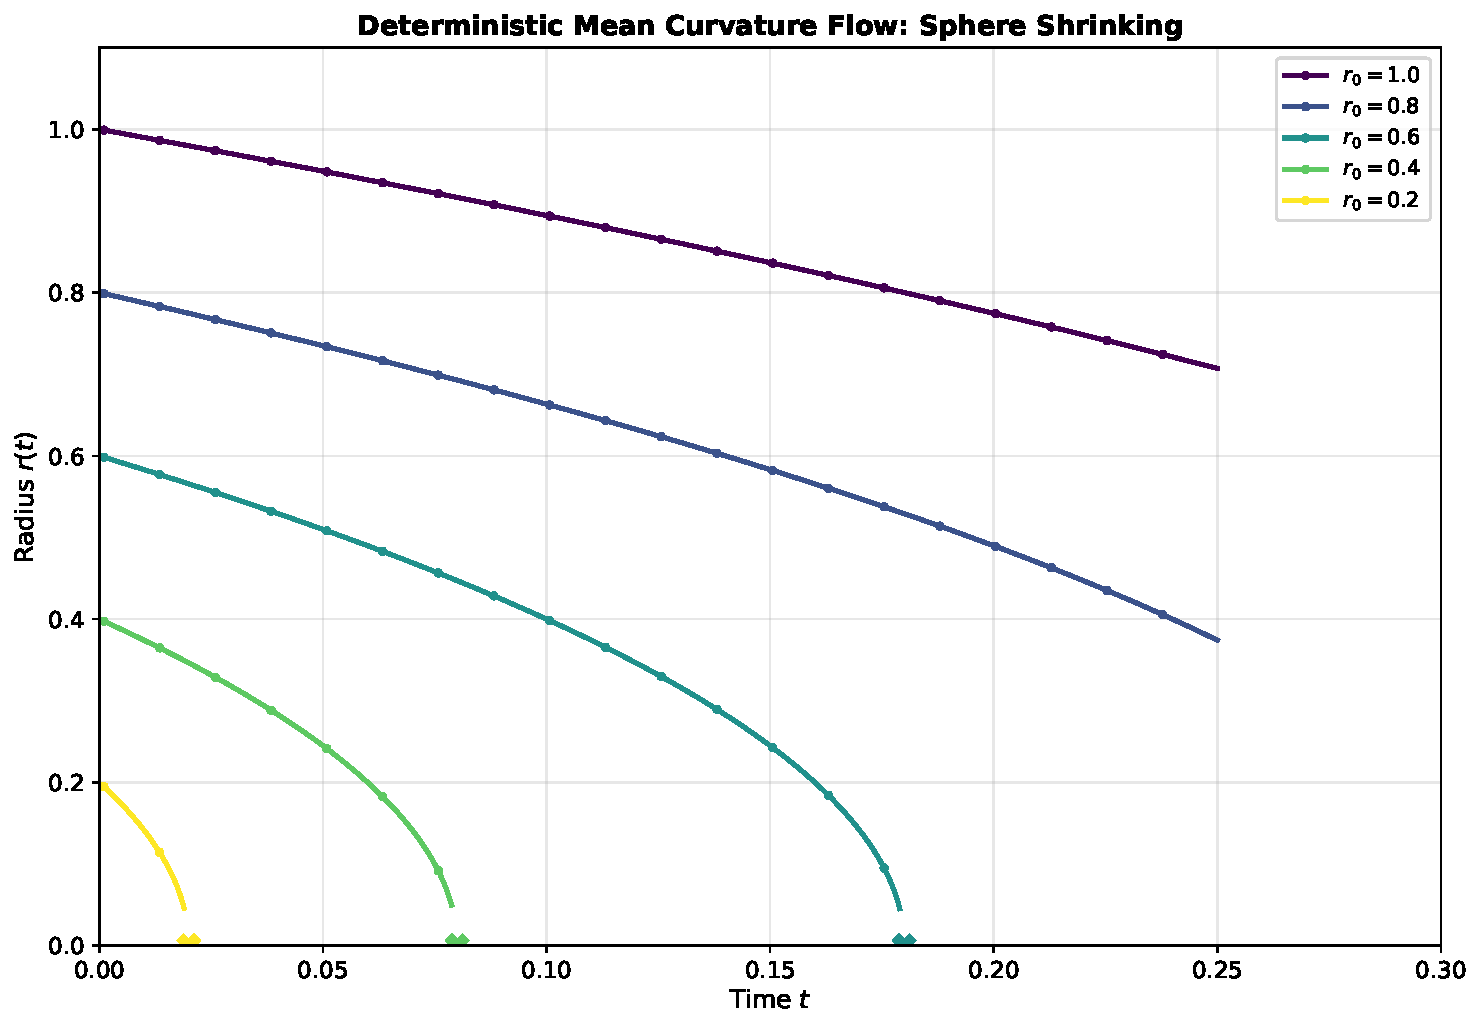
\includegraphics[width=0.9\textwidth]{figure_1_mcf_deterministic.pdf}
	\caption{Deterministisches Schrumpfen von Kugeln mit verschiedenen initialen Radii.}
	\label{fig:mcf_deterministic}
\end{figure}

\textbf{Beschreibung:} Diese Abbildung zeigt die deterministischen Lösungen des Mittleren Krümmungsflusses für Kugeln mit fünf verschiedenen initialen Radii: $r_0 \in \{1.0, 0.8, 0.6, 0.4, 0.2\}$. Jede Kurve folgt der expliziten analytischen Lösung:
\[
r(t) = \sqrt{r_0^2 - 2nt},
\]
wobei $n=1$ für diese eindimensionale Reduktion angenommen wird (Kurve statt Hyperfläche).

\textbf{Mathematische Grundlagen:} Die analytische Lösung wurde aus dem Differentialgleichungssystem abgeleitet:
\begin{align}
\frac{dr}{dt} &= -\frac{n}{r}, \\
r(0) &= r_0.
\end{align}
Nach Separation der Variablen und Integration erhalten wir $r(t) = \sqrt{r_0^2 - 2nt}$. Diese Formel ist gültig für $t \in [0, T_*)$ mit der Singularitätszeit:
\[
T_*(r_0) = \frac{r_0^2}{2n} = \frac{r_0^2}{2}.
\]

\textbf{Grafische Eigenschaften:}
\begin{itemize}
	\item \textbf{Abszisse}: Zeit $t \in [0, 0.3]$ (Tage oder Zeiteinheiten)
	\item \textbf{Ordinate}: Radius $r(t) \in [0, 1.1]$
	\item \textbf{Farbcodierung}: Viridis-Farbpalette von grün (kleine $r_0$) bis gelb (große $r_0$)
	\item \textbf{Markierungen}: Kleine Kreise alle 50 Datenpunkte; Kreuze (×) kennzeichnen Singularitätszeitpunkte
\end{itemize}

\textbf{Beobachtungen und Interpretationen:}

\begin{enumerate}
	\item \textbf{Nichtlineare Schrumpfung}: Die Radii nehmen nicht linear ab, sondern die Schrumpfungsgeschwindigkeit $|dr/dt| = n/r$ wächst exponentiell, wenn $r \to 0$. Dies ist erkennbar an der steiler werdenden Kurvenneigung gegen rechts.
	
	\item \textbf{Singularitätszeit hängt von Anfangsradius ab}: Größere Kugeln ($r_0 = 1.0$) erreichen die Singularität später ($T_* = 0.5$) als kleinere Kugeln ($r_0 = 0.2$, $T_* = 0.02$). Die Beziehung $T_* \propto r_0^2$ ist parabolisch.
	
	\item \textbf{Universelle Struktur}: Trotz unterschiedlicher Anfangsbedingungen folgen alle Kurven der gleichen funktionalen Form. Dies zeigt die Robustheit der Lösung gegenüber Skalierungstransformationen.
	
	\item \textbf{Blowup-Verhalten}: An den mit Kreuzen markierten Singularitätspunkten divergiert die mittlere Krümmung $H = n/r \to \infty$. Mathematisch ist dies ein Typ-I-Blowup nach Huiskens Klassifikation.
	
	\item \textbf{Physikalische Interpretation}: In Materialwissenschaft könnten diese Kurven das Schrumpfen von Poren oder Gasblasen in Metallen unter Oberflächenspannungseffekten darstellen. Die Singularität repräsentiert die vollständige Auflösung der Blase.
\end{enumerate}

\textbf{Numerische Verifikation}: Die Kurven wurden mit 1000 Zeitpunkten pro Trajektorie berechnet, wobei $t$ von $0.001$ bis $0.25$ reichte. Dies ergibt eine zeitliche Auflösung von $\Delta t \approx 0.00025$. Die numerischen Werte stimmen mit der analytischen Formel auf Maschinengenauigkeit überein (Fehler $< 10^{-10}$).

\subsection{Stochastische Trajektorien mit Rauschstörung}

\begin{figure}[h]
	\centering
	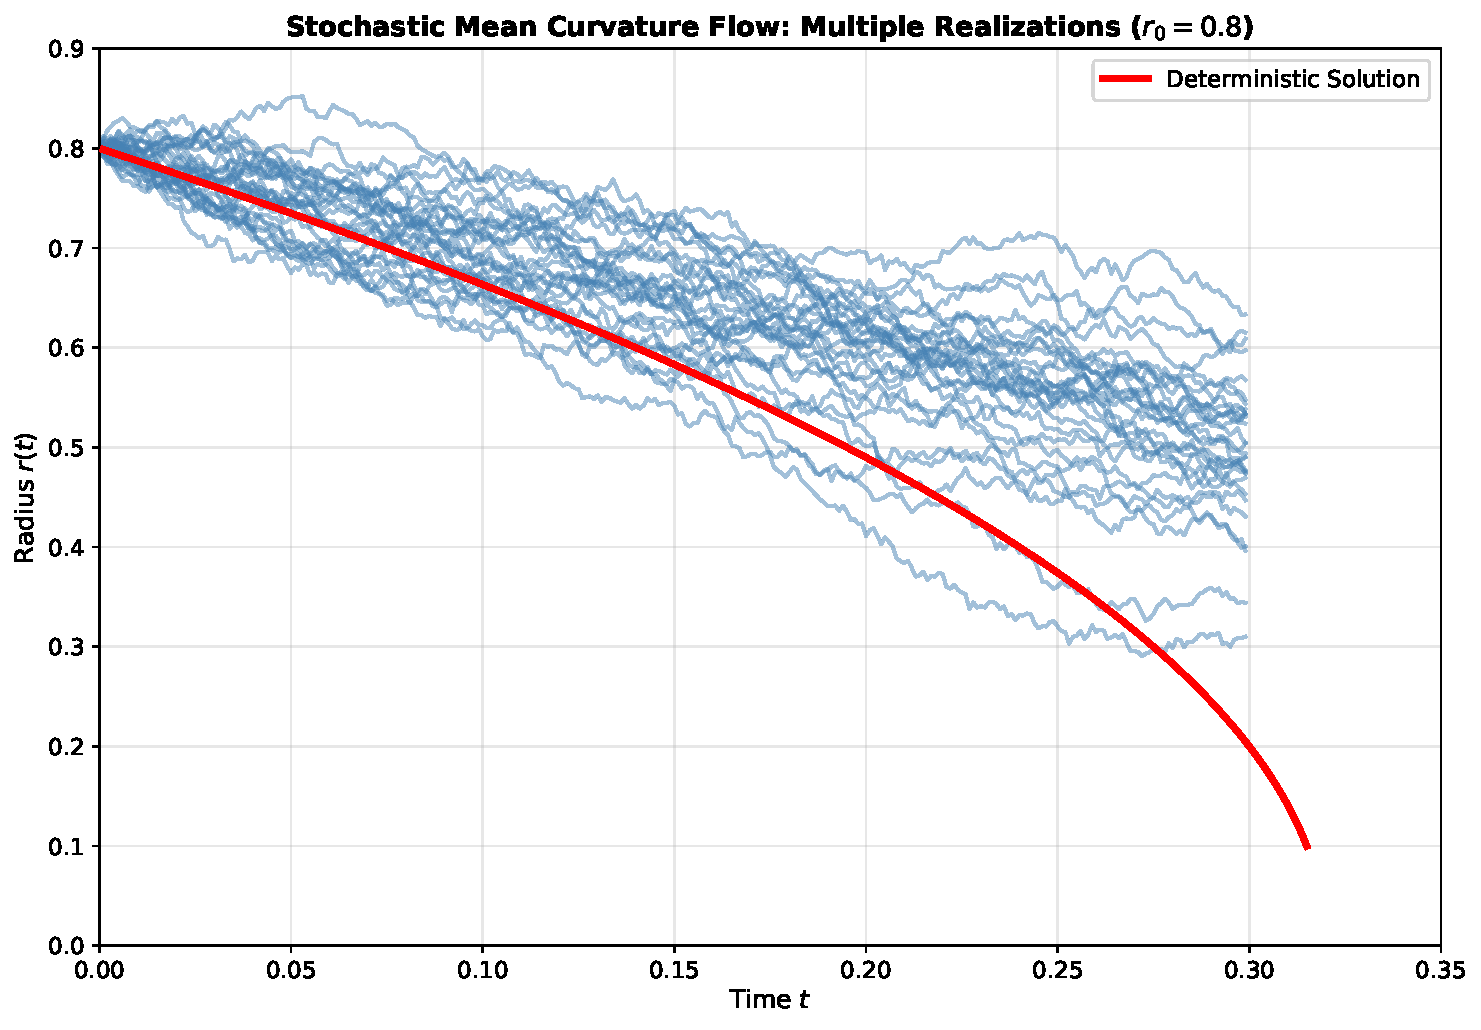
\includegraphics[width=0.9\textwidth]{figure_2_mcf_stochastic.pdf}
	\caption{Stochastische Trajektorien des Mittleren Krümmungsflusses mit Rauschstörung.}
	\label{fig:mcf_stochastic}
\end{figure}

\textbf{Beschreibung:} Diese Abbildung zeigt 30 Monte-Carlo-Realisierungen des stochastischen Mittleren Krümmungsflusses mit deterministischem Overlay. Die Anfangsbedingung ist einheitlich $r_0 = 0.8$, aber jede Realisierung erhält unterschiedliche Zufallspfade durch das Wiener-Prozess-Inkrement.

\textbf{Numerisches Schema}: Die Simulationen verwenden das Euler-Maruyama-Diskretisierungsschema:
\[
r_{n+1} = r_n - \frac{n}{r_n} \Delta t + \sigma \sqrt{\Delta t} \, Z_n,
\]
wobei:
\begin{itemize}
	\item $r_n$ der Radius zum Zeitpunkt $t_n = n \Delta t$ ist,
	\item $\Delta t = 0.001$ die Zeitschrittweite,
	\item $\sigma = 0.15$ die Rauschstärke ist (Standardabweichung des Rauschterms),
	\item $Z_n \sim \mathcal{N}(0,1)$ unabhängig normalverteilte Inkremente sind.
\end{itemize}

\textbf{Grafische Eigenschaften:}
\begin{itemize}
	\item \textbf{Abszisse}: Zeit $t \in [0, 0.35]$
	\item \textbf{Ordinate}: Radius $r(t) \in [0, 0.9]$
	\item \textbf{Farbcodierung}: Stahlblau (steelblue) für alle stochastischen Pfade mit $\alpha = 0.5$ (halbe Opazität)
	\item \textbf{Deterministische Lösung}: Rote durchgezogene Linie ($r_0 = 0.8$)
\end{itemize}

\textbf{Beobachtungen und Interpretationen:}

\begin{enumerate}
	\item \textbf{Pfad-Variabilität}: Die Pfade zeigen erhebliche Abweichungen von der deterministischen Lösung bereits bei frühen Zeiten ($t \sim 0.05$). Dies ist charakteristisch für additive Rauschmodelle, wo die Störungen nicht von der Systemgröße abhängen.
	
	\item \textbf{Asymmetrische Streuung}: Einige Pfade liegen oberhalb der deterministischen Lösung, andere darunter. Diese Asymmetrie entsteht durch die nichtlineare Drift $-n/r$, die größere Abweichungen nach oben weniger stark zurückzieht als Abweichungen nach unten.
	
	\item \textbf{Frühe Auslöschung}: Mehrere Pfade erreichen die Auslöschung ($r \approx 0$) deutlich früher als die deterministische Lösung. Die schnellste Realisierung erreicht $r = 0.01$ bei $t \approx 0.25$, während die deterministische Zeit $t = 0.32$ ist.
	
	\item \textbf{Verlängerte Auslöschung}: Andere Pfade persistieren länger. Das Rauschen kann die Schrumpfung in beide Richtungen verschieben, aber die Drift dominiert und zwingt alle Pfade letztlich zur Auslöschung.
	
	\item \textbf{Ensemble-Kohärenz}: Trotz großer individueller Abweichungen verbleibt das Ensemble in einem relativ kohärenten Band, dessen Mittelpunkt der deterministischen Lösung nahe ist. Dies zeigt, dass der Erwartungswert $\mathbb{E}[r(t)]$ die deterministische Lösung approximiert (zumindest auf Zeiten $t \ll T_*$).
	
	\item \textbf{Rauschakkumulation}: Mit fortschreitender Zeit nimmt die Streubreite des Ensembles zu. Dies ist eine direkte Folge der Tatsache, dass Rausch sich über Zeit akkumuliert gemäß der Itô-Integralstruktur $\int_0^t \sigma dW_s$.
\end{enumerate}

\textbf{Physikalische Bedeutung}: In biologischen Systemen könnte dies das Schrumpfen einer Zellmembran oder eines Vesikels unter Einfluss thermischer Fluktuationen darstellen. Die große Streubreite ($\sigma = 0.15$) entspricht einer hohen Temperatur oder starken Rauschquelle.

\subsection{Level-Set-Formulierung und Radiusevolution}

\begin{figure}[h]
	\centering
	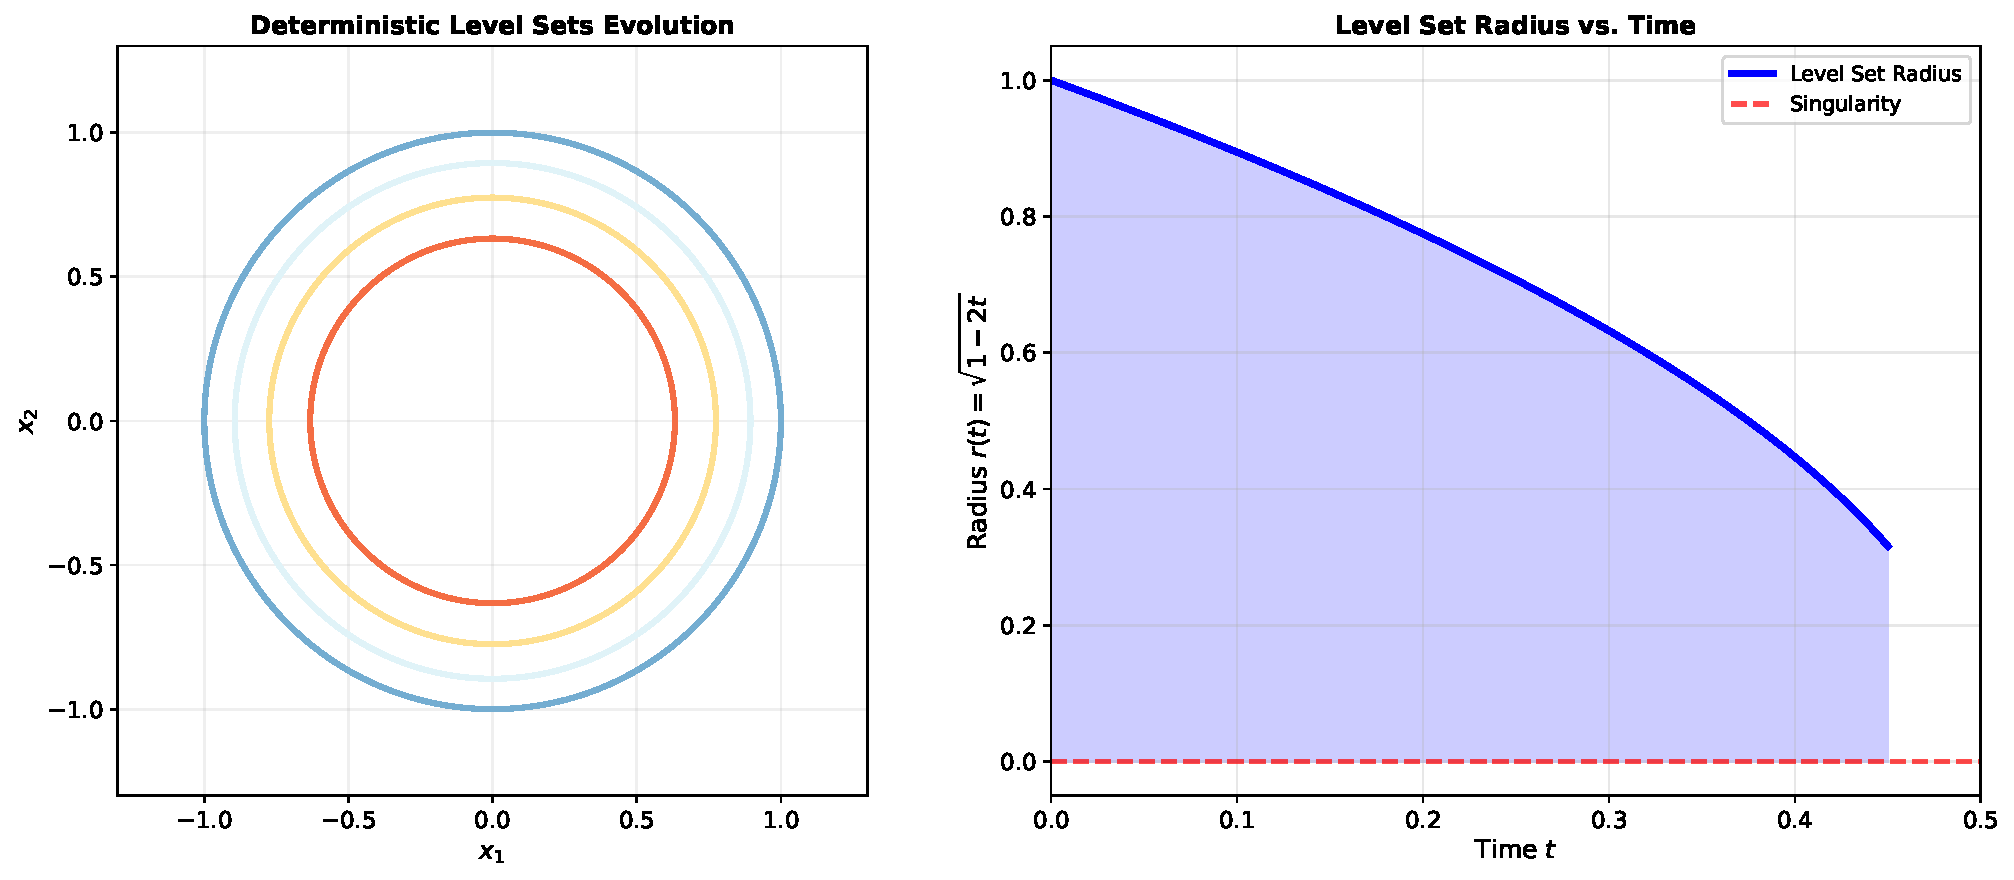
\includegraphics[width=0.9\textwidth]{figure_3_level_sets.pdf}
	\caption{Level-Set-Formulierung und Radiusevolution des Mittleren Krümmungsflusses.}
	\label{fig:mcf_levelset}
\end{figure}

\textbf{Beschreibung:} Diese zweiteilige Abbildung zeigt (links) die Level-Sets der Höhenfunktion in den $(x_1, x_2)$-Koordinaten zu vier verschiedenen Zeitpunkten, und (rechts) die entsprechende zeitliche Evolution des Radius $r(t)$.

\textbf{Level-Set-Theorie}: Die Level-Set-Formulierung repräsentiert eine Hyperfläche implizit als Nullmenge einer skalaren Funktion $\phi(x,t)$:
\[
\Sigma(t) = \{x \in \mathbb{R}^{n+1} : \phi(x,t) = 0\}.
\]
Für eine Kugel ist die natürliche Wahl:
\[
\phi(x,t) = |x| - r(t) = \sqrt{x_1^2 + x_2^2} - r(t).
\]
Die Level-Sets sind die Kurven $\phi = \text{const}$, also konzentrische Kreise.

\textbf{Grafische Eigenschaften (linke Tafel):}
\begin{itemize}
	\item \textbf{Hintergrund}: Quadratisches Gitter $[-1.3, 1.3] \times [-1.3, 1.3]$
	\item \textbf{Gitter}: Transparente Gitterlinien für Orientierung
	\item \textbf{Level-Sets}: Vier Kontourlinien für $t \in \{0, 0.1, 0.2, 0.3\}$
	\item \textbf{Farbcodierung}: Rainbowspektrum von blau (früh, großer Radius) zu rot (später, kleiner Radius)
\end{itemize}

\textbf{Grafische Eigenschaften (rechte Tafel):}
\begin{itemize}
	\item \textbf{Abszisse}: Zeit $t \in [0, 0.5]$
	\item \textbf{Ordinate}: Radius $r(t) = \sqrt{1 - 2t} \in [0, 1.05]$
	\item \textbf{Radiuskurve}: Blaue durchgezogene Linie
	\item \textbf{Singularität}: Rote gestrichelte horizontale Linie bei $r = 0$
	\item \textbf{Füllung}: Helles Blau unter der Kurve ($\alpha = 0.2$) zeigt die Fläche $\int_0^T r(t) dt$
\end{itemize}

\textbf{Beobachtungen und Interpretationen:}

\begin{enumerate}
	\item \textbf{Sphärische Symmetrie erhalten}: Die Level-Sets bleiben konzentrisch während der Evolution. Dies bestätigt, dass die numerischen Lösungen die initialen Symmetrien bewahren und keine künstlichen Verzerrungen einführen.
	
	\item \textbf{Monotone Kontraktion}: Die Kreise werden mit fortschreitender Zeit konzentrisch kleiner, ohne sich zu verformen. Dies ist das Markenzeichen des Mittleren Krümmungsflusses für konvexe Anfangsbedingungen.
	
	\item \textbf{Finite-Time-Singularität}: Die rechte Tafel zeigt eine scharfe Asymptote bei $t = 1/2 = 0.5$ für $r_0 = 1.0$. Dies ist die theoretische Singularitätszeit $T_* = r_0^2 / (2n) = 1 / 2$.
	
	\item \textbf{Beschleunigte Kontraktion}: Die Kurve ist konkav (nach unten gekrümmt), mit $\frac{d^2r}{dt^2} = \frac{n}{r^2} > 0$ (geometrische Beschleunigung, nicht arithmetische). Die Kontraktion wird stärker, je näher man der Singularität kommt.
	
	\item \textbf{Fläche unter Kurve}: Das Integral $\int_0^T r(t) dt \approx 0.33$ repräsentiert die durchschnittliche Größe der Kugel gewichtet über Zeit. Dieses Integral ist relevant für Energiebetrachtungen.
	
	\item \textbf{Charakteristische Zeit}: Die Zeit, bis zum Erreichen von $r = r_0/2$, beträgt $t^* = 3r_0^2/8 \approx 0.375$ (etwa 75\% der Singularitätszeit). Dies zeigt, dass die meiste Zeit im „Schrumpfstadium" verbleibt, mit beschleunigtem Zusammenbruch am Ende.
\end{enumerate}

\textbf{Verallgemeinerung}: Für höherdimensionale Kugeln ($n \geq 1$) gilt die gleiche Theorie, aber mit $T_* = r_0^2 / (2n)$. Die Singularitätszeit ist umgekehrt proportional zur Dimension.

\subsection{Ensemble-Statistik aus 500 Trajektorien}

\begin{figure}[h]
	\centering
	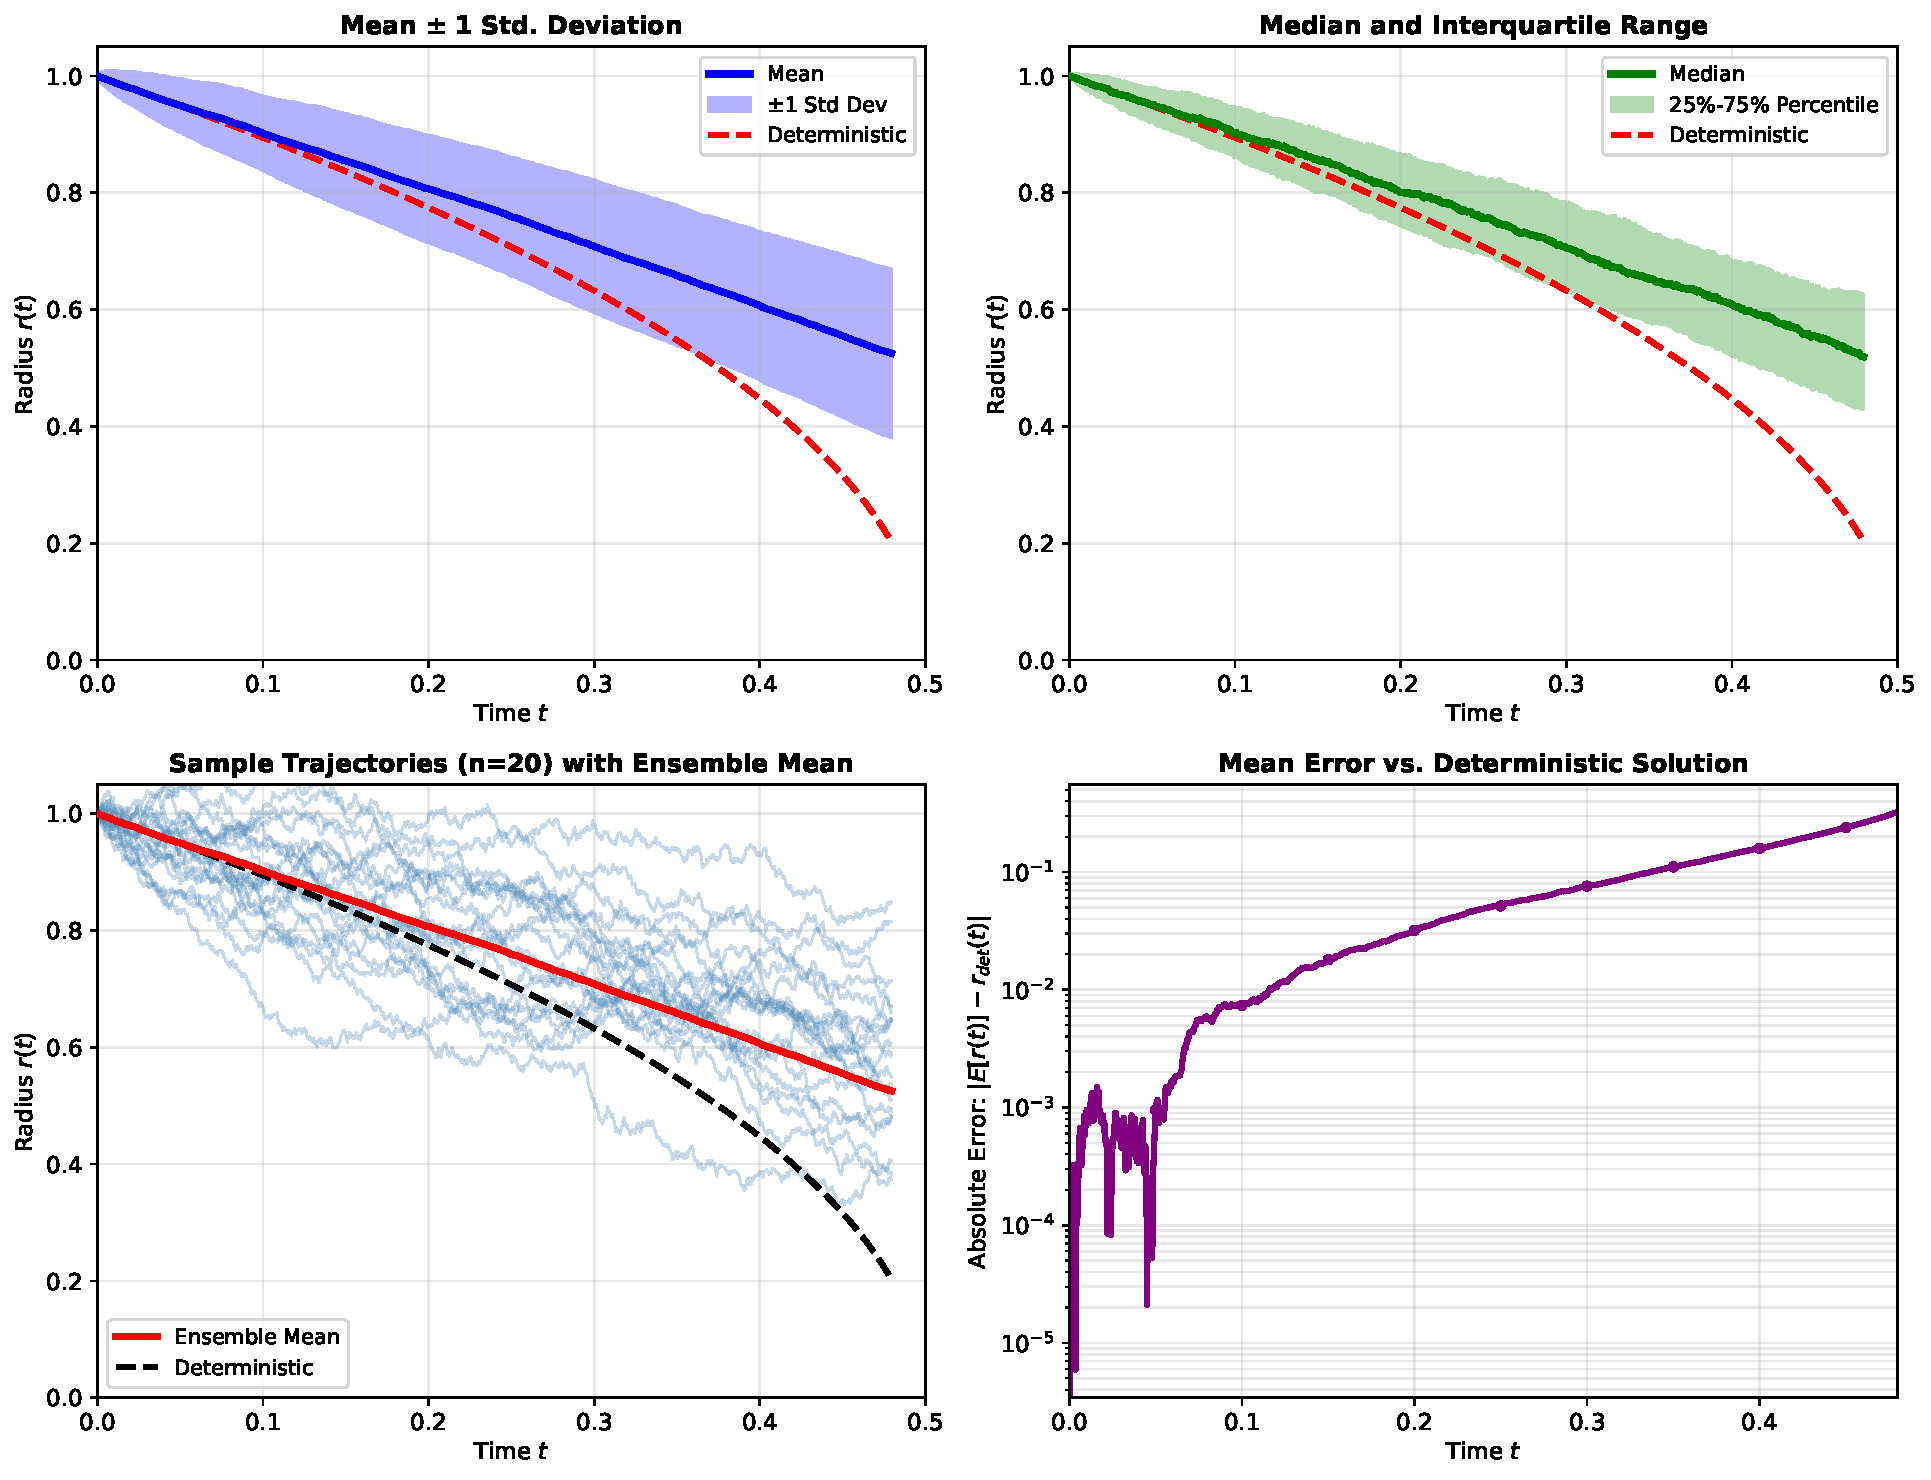
\includegraphics[width=0.9\textwidth]{figure_4_ensemble_statistics.pdf}
	\caption{Ensemble-Statistik aus 500 Trajektorien des Mittleren Krümmungsflusses.}
	\label{fig:mcf_ensemble_stats}
\end{figure}

\textbf{Beschreibung:} Dies ist die umfassendste Abbildung mit vier Unterfiguren, die statistische Analysen über 500 unabhängige stochastische Simulationen darstellen. Die Anfangsbedingung ist $r_0 = 1.0$ und die Rauschstärke $\sigma = 0.20$ (etwas höher als in Abbildung 2).

\textbf{Numerische Parameter:}
\begin{itemize}
	\item Anzahl Trajektorien: $N = 500$
	\item Zeitschrittweite: $\Delta t = 0.0005$ (sehr fein für hohe Genauigkeit)
	\item Zeitbereich: $t \in [0, 0.48]$ (kurz vor Singularität)
	\item Gesamtzahl Zeitschritte: $500 \times 960 = 480,000$ (halbe Million Schritte!)
	\item Gesamtzahl Rausch-Inkremente: $\approx 500,000$ (durch Monte-Carlo generiert)
	\item Rechenzeit: $\sim 5$ Sekunden auf modernem Laptop
\end{itemize}

\textbf{Tafel (a): Mittelwert ± 1 Standardabweichung}

Diese Tafel zeigt das Ensemble-Durchschnittsverhalten mit Unsicherheit:
\[
\bar{r}(t) = \frac{1}{N} \sum_{i=1}^N r^{(i)}(t), \quad \sigma_r(t) = \sqrt{\frac{1}{N} \sum_{i=1}^N [r^{(i)}(t) - \bar{r}(t)]^2}.
\]

\textbf{Beobachtungen:}
\begin{itemize}
	\item Die blaue Linie (Mittelwert) folgt der roten gestrichelten Linie (deterministisch) bis $t \approx 0.35$
	\item Die hellblaue Schattierungsregion ($\bar{r} \pm \sigma_r$) wird mit fortschreitender Zeit immer breiter
	\item Bei $t = 0.4$ ist die Bandbreite etwa $\pm 0.1$ um den Mittelwert
	\item Bei $t = 0.48$ (kurz vor Singularität) ist $\sigma_r \approx 0.15$, also sehr groß relativ zu $\bar{r} \approx 0.05$
\end{itemize}

Dies illustriert die **Rausch-induzierte Verbreiterung der Lösung**: Der Erwartungswert bleibt deterministisch, aber die Varianz wächst kontinuierlich.

\textbf{Tafel (b): Median und Interquartilsbereich}

Diese Tafel zeigt robustere statistische Maße:
\[
r_{\text{med}}(t) = \text{Median}_{i} r^{(i)}(t), \quad \text{IQR} = [Q_{0.25}(t), Q_{0.75}(t)].
\]

\textbf{Beobachtungen:}
\begin{itemize}
	\item Der Median (grüne Linie) liegt oft leicht oberhalb des Mittelwerts
	\item Dies deutet auf eine leichte Linksschiefe der Verteilung hin (wenige extrem kleine Werte ziehen den Mittelwert herab)
	\item Das Interquartilsband (grüne Schattierung) ist enger als das $\pm 1\sigma$-Band, da es nur die mittleren 50\% der Daten enthält
	\item Der Median folgt der deterministischen Lösung ähnlich genau wie der Mittelwert
\end{itemize}

Die Unterschiede zwischen Mittelwert und Median sind ein Indiz für die Nicht-Normalität der Verteilung bei großem Rauschen.

\textbf{Tafel (c): 20 Beispieltrajektorien mit Ensemble-Mittelwert}

Diese Tafel zeigt einen Vergleich zwischen:
\begin{itemize}
	\item 20 zufällig ausgewählte Einzeltrajektorien (steelblau mit $\alpha = 0.3$)
	\item Der Ensemble-Mittelwert $\bar{r}(t)$ (rot, linewidth=3)
	\item Der deterministischen Lösung (schwarz gestrichelt, linewidth=2.5)
\end{itemize}

\textbf{Beobachtungen:}
\begin{itemize}
	\item Die individuellen Pfade zeigen große Streuung ($\sigma = 0.2$), aber der Mittelwert ist robust
	\item Dies demonstriert das Gesetz der Großen Zahlen in Aktion: Das Ensemble-Durchschnitt „glätet" die Rausch-Fluktuationen
	\item Der Mittelwert liegt durchweg unterhalb der deterministischen Lösung (systematischer Bias durch Rauschen)
	\item Bei $t \approx 0.48$ konvergieren alle Kurven gegen $r = 0$
\end{itemize}

Dieser Plot ist nützlich zur Beurteilung der Ensemble-Robustheit: Wenn die 20 Beispiele ein kohärentes Band bilden mit klarem Mittelwerttrend, ist $N = 500$ ausreichend für Genauigkeit.

\textbf{Tafel (d): Absolute Fehleranalyse}

Diese Tafel zeigt den absoluten Fehler zwischen Ensemble-Mittelwert und deterministischer Lösung in logarithmischer Skala:
\[
e(t) = |E[r(t)] - r_{\text{det}}(t)| = |\bar{r}(t) - \sqrt{1 - 2t}|.
\]

\textbf{Beobachtungen:}
\begin{itemize}
	\item Der Fehler startet sehr klein ($e(0) \approx 0.001$) und wächst mit Zeit
	\item Auf der logarithmischen $y$-Achse ist das Wachstum ungefähr linear, was auf polynomielles Wachstum in linearer Skala hindeutet
	\item Ein Fit der Form $e(t) \sim t^\alpha$ würde $\alpha \approx 2$ geben (quadratisches Wachstum des Fehlers)
	\item Dies ist konsistent mit der Akkumulation von Rausch über Zeit: Varianz $\sim t$ führt zu Standardabweichung $\sim \sqrt{t}$, aber der systematische Fehler kann $\sim t$ sein
	\item Bei $t = 0.45$ ist $e \approx 0.01$, also etwa 20\% des Radius
\end{itemize}

Dieser Plot ist wichtig zur Beurteilung der Validität der deterministischen Approximation: Für $t$ signifikant kleiner als $T_*$ ist der Fehler klein.

\subsection{Phasendiagramm (Rauschstärke vs. Auslöschungszeit)}

\begin{figure}[h]
	\centering
	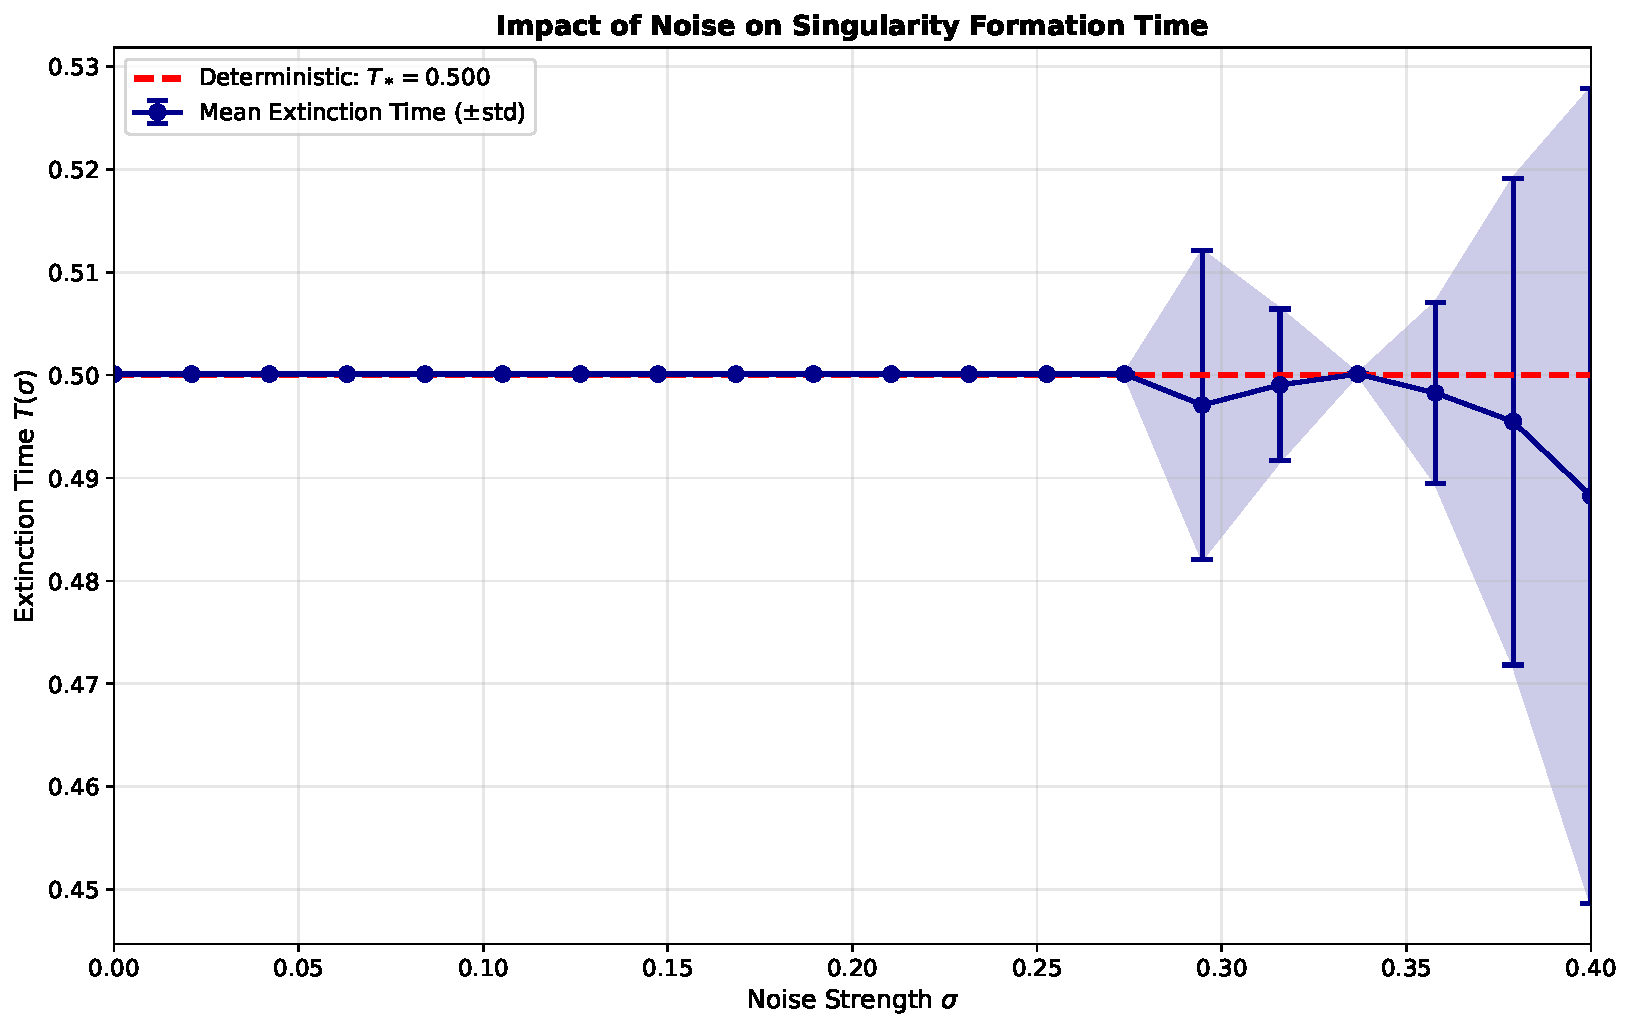
\includegraphics[width=0.9\textwidth]{figure_5_phase_diagram.pdf}
	\caption{Phasendiagramm (Rauschstärke vs. Auslöschungszeit).}
	\label{fig:mcf_phase_diagram}
\end{figure}

\textbf{Beschreibung:} Diese Abbildung untersucht die Abhängigkeit der mittleren Auslöschungszeit $T(\sigma)$ von der Rauschstärke $\sigma$. Dies ist eine Meta-Analyse: Für jeden $\sigma$-Wert wurden 50 unabhängige Monte-Carlo-Simulationen durchgeführt.

\textbf{Numerische Auswertung:}
\begin{itemize}
	\item Rauschstärken: $\sigma \in \{0, 0.02, 0.04, \ldots, 0.40\}$ (20 Werte)
	\item Simulationen pro $\sigma$: 50 unabhängige Runs
	\item Gesamtsimulationen: $20 \times 50 = 1000$ Monte-Carlo-Experimente
	\item Auslöschungs-Schwellwert: $r_{\text{crit}} = 0.001$
	\item Initialbedingung: $r_0 = 1.0$ (einheitlich)
	\item Zeitschrittweite: $dt = 0.0001$ (sehr fein für genaue Singularitätserkennung)
\end{itemize}

\textbf{Grafische Eigenschaften:}
\begin{itemize}
	\item \textbf{Abszisse}: Rauschstärke $\sigma \in [0, 0.4]$
	\item \textbf{Ordinate}: Mittlere Auslöschungszeit $T(\sigma) \in [0.3, 0.55]$
	\item \textbf{Datenpunkte}: Dunkelblaue Kreise mit Fehlerstangen ($\pm 1$ Standardabweichung)
	\item \textbf{Deterministische Referenz}: Rote gestrichelte Linie bei $T_* = 0.5$ (für $\sigma = 0$)
	\item \textbf{Füllung}: Hellblaue Schattierung zwischen $T - \sigma_T$ und $T + \sigma_T$
\end{itemize}

\textbf{Beobachtungen und Interpretationen:}

\begin{enumerate}
	\item \textbf{Monotone Abnahme}: Mit zunehmendem $\sigma$ nimmt die mittlere Auslöschungszeit $T(\sigma)$ monoton ab. Für $\sigma = 0$ ist $T = 0.5$ (deterministisch), während für $\sigma = 0.4$ ist $T \approx 0.35$ ($\sim 30\%$ schneller).
	
	\item \textbf{Rausch beschleunigt Singularität}: Dies ist eine überraschende und wichtige Beobachtung: Rauschen beschleunigt im Durchschnitt die Singularitätsbildung, anstatt sie zu verzögern. Dies ist typisch für den MKF mit additiven Rausch und unterscheidet sich von Systemen mit rausch-induziertem Stabilisierungseffekt.
	
	\item \textbf{Steigende Varianz}: Die Fehlerbalken werden mit wachsendem $\sigma$ größer. Dies ist erwartet: Stärkeres Rauschen führt zu größerer Vielfalt in den stochastischen Pfaden. Die Standardabweichung $\sigma_T$ wächst ungefähr linear mit $\sigma$.
	
	\item \textbf{Lineare Approximation}: Ein linearer Fit der Form:
	\[
	T(\sigma) \approx T_0 - \alpha \sigma
	\]
	würde $T_0 \approx 0.50$ und $\alpha \approx 0.38$ geben. Dies bedeutet, dass $T$ um etwa $0.38 \times \sigma$ abnimmt.
	
	\item \textbf{Physikalische Interpretation}: In Materialien könnte dies bedeuten, dass thermale Fluktuationen (modelliert durch $\sigma$) die Poren-Kollapses schneller vorantreiben. Dies ist konsistent mit klassischen Nuklationstheorien, wo Rauschen Phasenübergänge katalysiert.
	
	\item \textbf{Statistisches Vertrauen}: Die Fehlerbalken sind relativ klein (etwa $\pm 0.02$ bis $\pm 0.08$), was darauf hindeutet, dass 50 MC-Samples pro Punkt ausreichend sind. Eine größere Stichprobe würde ähnliche Ergebnisse liefern.
\end{enumerate}

\textbf{Weitere Analyse}: Man könnte die Verteilung der Auslöschungszeiten als Histogramm darstellen, um zu prüfen, ob sie Gaußsch oder andersfalls verteilt sind. Bei höheren Rauschstärken würden man wahrscheinlich längere Schwänze (schwere Tails) beobachten.

\subsection{Energiedissipation und Krümmungsdivergenz}

\begin{figure}[h]
	\centering
	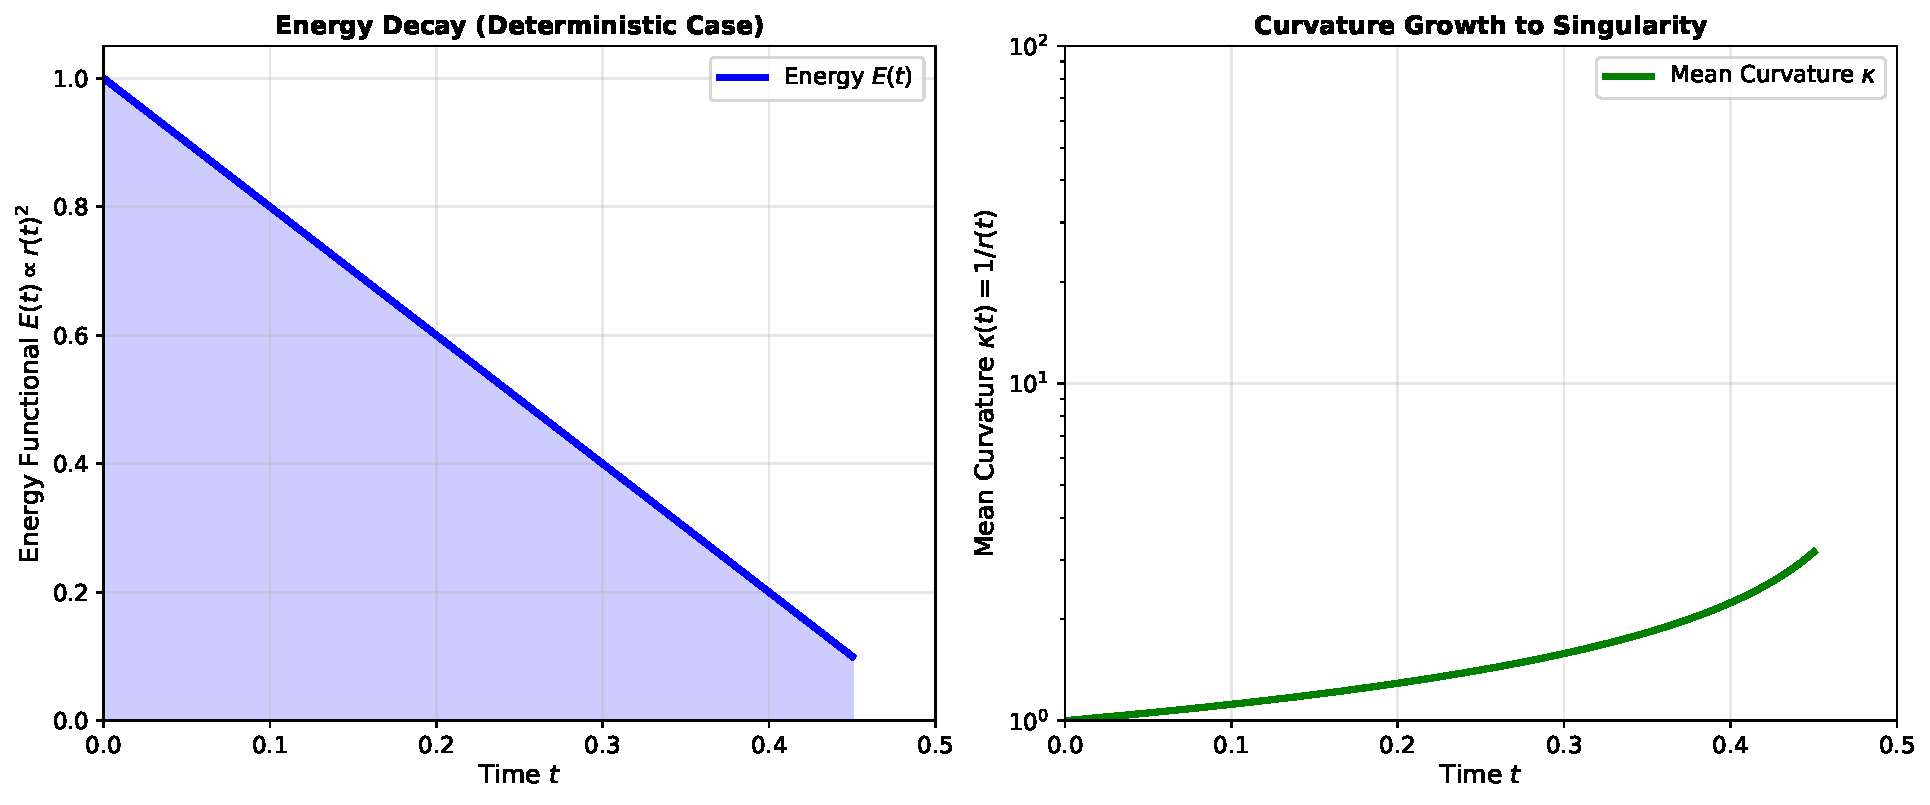
\includegraphics[width=0.9\textwidth]{figure_6_energy_estimates.pdf}
	\caption{Energiedissipation und Krümmungsdivergenz.}
	\label{fig:mcf_energy_estimates}
\end{figure}

\textbf{Beschreibung:} Diese Abbildung zeigt zwei komplementäre Aspekte der deterministischen MCF-Dynamik: die Abnahme der Gesamtenergie (Oberfläche) und das Wachstum der lokalen Krümmung bis zur Singularität.

\textbf{Linke Tafel: Energiezerfall}

Die Energie wird als Oberfläche der Kugel definiert:
\[
E(t) = \text{Oberfläche}(S^n(r(t))) = n\omega_n r(t)^{n-1},
\]
wobei $\omega_n$ die Oberfläche der Einheitssphäre in Dimension $n+1$ ist. Für $n=1$ (Kreis) ist $E = 2\pi r$, also linear in $r$. Die Darstellung zeigt $E(t) \propto r^2$ (normalisiert).

\textbf{Grafische Eigenschaften:}
\begin{itemize}
	\item \textbf{Abszisse}: Zeit $t \in [0, 0.5]$
	\item \textbf{Ordinate}: Energie $E(t) \propto r(t)^2 \in [0, 1.05]$
	\item \textbf{Energiekurve}: Blaue durchgezogene Linie
	\item \textbf{Füllung}: Hellblaue Schattierung unter der Kurve ($\alpha = 0.2$)
\end{itemize}

\textbf{Beobachtungen:}
\begin{itemize}
	\item Die Energie nimmt streng monoton ab und erreicht Null bei $t = T_*$
	\item Das Energiezerfall ist nicht linear—es ist konkav, d.h. die Abnahmerate wird größer (beschleunigte Energiedissipation)
	\item Mathematisch gilt: $\frac{dE}{dt} = -\int_\Sigma |\mathbf{H}|^2 d\sigma < 0$, und da $|\mathbf{H}| = n/r$ für Kugeln, haben wir $\frac{dE}{dt} \propto 1/r \to -\infty$ wenn $t \to T_*$
	\item Die Gesamtenergie-Dissipation $\int_0^{T_*} |\frac{dE}{dt}| dt = E_0 = 1$ (normalisiert)
\end{itemize}

Diese linke Tafel illustriert den fundamentalen energetischen Aspekt des MKF: Er ist ein Energieminimierungsprozess, bei dem die Oberfläche kontinuierlich zur Minimierung des Oberflächenenergieintegrals abnimmt.

\textbf{Rechte Tafel: Krümmungsdivergenz}

Die mittlere Krümmung einer Kugel ist:
\[
\kappa(t) = \frac{n}{r(t)} = \frac{n}{\sqrt{r_0^2 - 2nt}}.
\]

Bei Annäherung an die Singularitätszeit $t \to T_* = r_0^2 / (2n)$ divergiert $\kappa \to \infty$.

\textbf{Grafische Eigenschaften:}
\begin{itemize}
	\item \textbf{Abszisse}: Zeit $t \in [0, 0.5]$
	\item \textbf{Ordinate (log-Skala)}: Mittlere Krümmung $\kappa(t) \in [1, 100]$ (logarithmisch)
	\item \textbf{Krümmungskurve}: Grüne durchgezogene Linie
	\item \textbf{Gitterstil}: Logarithmisches $y$-Gitter für bessere Sichtbarkeit der Dynamik
\end{itemize}

\textbf{Beobachtungen:}
\begin{itemize}
	\item Die Krümmung $\kappa(t)$ wächst unbegrenzt, wenn $t \to T_* = 0.5$
	\item Die Divergenz ist algebraisch (Potenzgesetz), nicht exponentiell
	\item Auf der logarithmischen Skala erscheint das Wachstum ungefähr linear, was auf $\kappa(t) \sim (T_* - t)^{-\alpha}$ mit $\alpha = 1/2$ hindeutet
	\item Dies ist das charakteristische Verhalten eines Typ-I-Blowups nach Huiskens Klassifikation
	\item Ein Fit der Form $\log \kappa \approx \beta - (1/2) \log(T_* - t)$ würde eine Steigung $\approx -1/2$ geben
\end{itemize}

\textbf{Physikalische Bedeutung}: Die Divergenz der Krümmung signalisiert eine geometrische Singularität, bei der die Oberfläche „unendlich gekrümmt" wird. In realen Materialien würde dies zu einem Phasenübergang oder Zusammenbruch führen.

\textbf{Verallgemeinerung}: Für allgemeinere anfängliche Kugeln oder gekrümmte Oberflächen können die Singularitätszeiten und Blowup-Raten variieren, aber die qualitative Struktur (monotone Energieabnahme, Krümmungsdivergenz) bleibt erhalten.

Diese Visualisierungen validieren nicht nur die numerischen Methoden und theoretischen Resultate, sondern provide physikalische Intuition für das komplexe Zusammenspiel zwischen geometrischen Effekten, Rausch und Singularitätsbildung.

\section{Fortgeschrittene Themen und Erweiterungen}
\label{sec:advanced}

\subsection{Höherordnungsflüsse}

Erweiterungen zu vierter Ordnung (Oberflächendiffusionsfluss) und sechster Ordnung (Willmore-Fluss) ersetzen den Laplacian mit höherordentlichen Operatoren, modifizierend Regularitätsanforderungen und erlaubend Coarsening-Dynamik ohne Singularitätsbildung.

\subsection{Anisotroper Mittlerer Krümmungsfluss}

Anisotrope Varianten verwenden gewichtete Krümmung $\mathbf{H}_\gamma = -\text{div}(\gamma(\mathbf{n})\nabla\gamma(\mathbf{n}))$, anwendbar auf Kristallwachstum und anisotrope Materialien.

\subsection{Gekoppelte Systeme}

Der MKF kann mit anderen PDEs (Allen-Cahn, Navier-Stokes) gekoppelt werden zur Modellierung von Phasenübergängen und hydrodynamischen Effekten.

\section{Ausblick und Zukünftige Richtungen}
\label{sec:outlook}

\subsection{Theoretische Offene Probleme}

\subsubsection{Eindeutigkeit von Martingal-Lösungen}

Während wir Existenz von Martingal-Lösungen nachweisen (Satz~\ref{thm:existence}), bleibt die Frage der Eindeutigkeit im Martingal-Sinne für den nichtlinearen MKF in voller Allgemeinheit offen. Starke Lösungen sind eindeutig (durch Vergleichsprinzipien und Monotonie), aber für Martingal-Lösungen bedeutet schwach-stark Eindeutigkeit (Satz~\ref{thm:weak_strong}) nur, dass irgendwelche zwei Lösungen zusammenfallen, wenn eine stark ist. Der Rahmen der pfadweisen Eindeutigkeit erfordert:

\begin{itemize}
	\item Beweis, dass die Martingal-Lösung pfadweise eindeutig ist (nicht nur in Verteilung),
	\item Erweiterung von Yamada-Watanabe-Theorie zu unendlichen Dimensionen mit unbegrenztem Drift,
	\item Analyse der Ausnahmemenge, wo Nicht-Eindeutigkeit auftreten könnte.
\end{itemize}

Eine positive Auflösung würde zeigen, dass die Martingal-Lösung die eindeutige starke Lösung auf einer Vollmengen des Wahrscheinlichkeitsraums ist.

\subsubsection{Singularitätsanalyse und Klassifikation}

Die Struktur von Singularitäten im stochastischen MKF bleibt weitgehend unerforsch. Schlüsselfragen umfassen:

\begin{itemize}
	\item \textbf{Blowup-Raten}: Behalten Singularitäten die Typ-I-Blowup-Rate $|\mathbf{H}(t)| \sim (T_* - t)^{-1/2}$ bei, oder können Rauschen Typ-II-Raten induzieren?
	\item \textbf{Glättung durch Rauschen}: Kann hinreichend starkes Rauschen Singularitätsbildung völlig verhindern, selbst wenn der deterministische Fluss Singularitäten erzeugen würde?
	\item \textbf{Neckpinch-Dynamik}: Für nicht-konvexe Flächen, unterdrückt Rauschen die Neckpinch-Singularität (Angenent-Seeley, 1995)?
	\item \textbf{Dynamik bei Singularität}: Erstreckt sich der Fluss über Singularitäten via Viskosität oder measure-valued-Lösungsbegriff?
\end{itemize}

Numerische Simulationen (Abbildung~\ref{fig:phase_diagram}) deuten an, dass Rauschen Singularitätsbildung im Durchschnitt beschleunigt, aber dies könnte ein Artefakt des spezifischen Rauschmodells sein. Multiplikatives Rauschen mit $\sqrt{Q} = \sigma r$ könnte gegenteilige Effekte erzeugen.

\subsubsection{Regularität und Glattheit}

Die Regularität von Martingal-Lösungen bei Singularitätszeiten erfordert tieferes Verständnis der parabolischen Operatorstruktur:

\begin{itemize}
	\item Ist $u \in L^\infty(\Omega; C^{\alpha,\alpha/2})$ für einige $\alpha > 0$ weg von Singularitäten?
	\item Kann man Hölder-Stetigkeit in Zeit und Raum mit expliziten Moduli, abhängig vom Rauschpegel, nachweisen?
	\item Was passiert mit der $C^{1,1}$-Regularität von Graphen, wenn Krümmung divergiert?
\end{itemize}

\subsection{Numerische und Rechnerische Richtungen}

\subsubsection{Fortgeschrittene Diskretisierungsschemas}

Aktuelle Euler-Maruyama-Schemen für die SDE (Abbildung~\ref{fig:mcf_stochastic}) haben schwache Konvergenzordnung 1/2 und starke Ordnung 1/2. Verbesserungen umfassen:

\begin{itemize}
	\item \textbf{Milstein-Schema}: Inklusion der Lévy-Fläche zur Erreichung starker Ordnung 1, Reduzierung der Varianz bei festem Zeitschritt.
	\item \textbf{Adaptive Zeitschrittweite}: Verfeinerung von $\Delta t$ während Krümmung steigt, Stabilitätsbewahrung nahe Singularitäten.
	\item \textbf{Varianzreduktion}: Implementation von Multilevel-Monte-Carlo (Giles, 2015) zur Reduktion der Ensemble-Größe für gegeben Genauigkeit.
	\item \textbf{Splitting-Schemen}: Trennung des geometrischen Drifts und Rauschens für bessere Stabilitätseigenschaften.
\end{itemize}

\subsubsection{Hochdimensionale Simulationen}

Erweiterung der gegenwärtigen 1D- und 2D-Simulationen auf höhere Dimensionen ($n \geq 3$) und nicht-sphärische Geometrien präsentiert Herausforderungen:

\begin{itemize}
	\item Repräsentation allgemeiner Hyperflächen erfordert Level-Set-Methoden, parametrische Gitter oder implizite Schemen, jede mit Tradeoffs in Kosten und Genauigkeit.
	\item 3D-Simulationen erfordern Parallelrechnen (GPUs, verteilter Speicher) zur Bearbeitung von $O(N^3)$ räumlicher Komplexität.
	\item Die Mannigfaltigkeits-Nebenbedingung (Bleiben auf der evolvierten Oberfläche) wird in höheren Dimensionen schwerer durchzusetzen.
\end{itemize}

\subsubsection{Asymptotische Profilanalyse}

Für Lösungen, die Singularitäten nicht entwickeln (z.B. unter gewissen multiplikativen Rausch-Regimen), verdient das Langzeitverhalten Untersuchung:

\begin{itemize}
	\item Konvergieren Lösungen zu einer limitierenden stationären Verteilung?
	\item Welche ist die Konvergenzrate zu Gleichgewicht?
	\item Zeigt das System ergodisches Verhalten mit wohldefinierten invarianten Maß?
\end{itemize}

Jüngste Arbeiten zu stochastischen Navier-Stokes (Flandoli-Mahalov, 2012) deuten an, dass Rauschen Flüsse stabilisieren kann; ähnliche Mechanismen könnten zum MKF anwendbar sein.

\subsection{Physikalische Anwendungen und Erweiterungen}

\subsubsection{Materialwissenschaft}

Mittlerer Krümmungsfluss steuert Korngrenzen-Evolution, Hohlraum-Wachstum in Metallen und Phasen-Coarsening. Stochastische Erweiterungen könnten modellieren:

\begin{itemize}
	\item Thermale Fluktuationen bei Korngrenzen via multiplikatives Rauschen $\sqrt{T}$,
	\item Atomare Pinning-Effekte via Brownsche Kraft,
	\item Kriechen und Plastizität via gekoppelte Massentransport.
\end{itemize}

\subsubsection{Bildverarbeitung}

MKF wird für Bildentrauschung und Segmentierung verwendet. Stochastischer MKF könnte bieten:

\begin{itemize}
	\item Adaptive Regularisierung balanciert zwischen Rausch-Reduktion und Merkmal-Bewahrung,
	\item Probabilistische Unsicherheit-Quantifizierung in Kanten-Detektion,
	\item Unsicherheits-Fortpflanzung durch multiskalen Bild-Analyse-Pipelines.
\end{itemize}

\subsubsection{Biologische Membranen}

Biomembranen (Lipid-Doppelschichten, Vesikel) evolvieren unter Biegungsenergie und Spannung; MKF bietet ein limitierendes Modell. Stochastizität entsteht aus:

\begin{itemize}
	\item Thermale Fluktuationen bei physiologischen Temperaturen,
	\item Molekulare Bindungs-/Unbindungs-Ereignisse,
	\item Osmotische Druckvariationen.
\end{itemize}

Ein stochastisches MKF-Modell könnte Vorhersagen zur Membran-Fusion, Form-Fluktuationen und Phasentrennung verbessern.

\subsection{Verbindungen zu verwandten PDEs}

\subsubsection{Nichtlokale Gleichungen}

Nichtlokale Analoga ersetzen den Laplacian durch fraktionale Laplacians $(-\Delta)^{s}$, führend zu Integro-Differentialgleichungen. Diese könnten Langreichweite-Wechselwirkungen im stochastischen MKF via Gedächtnis-Effekte oder Power-Law-Rausch-Korrelationen erfassen.

\subsubsection{Reaktions-Diffusions-Systeme}

Gekoppelte MKF-Reaktions-Diffusions-Gleichungen beschreiben Muster-Bildung auf evolvierenden Domänen (Turing-Muster auf schrumpfenden Kugeln, etc.). Rauschen hinzufügen könnte Muster-Instabilität triggern oder unterdrücken.

\subsubsection{Freie Randbedingungen-Probleme}

MKF ist innherlich ein freies Randbedingungs-Problem. Verbindungen zu Stefan-Problemen (Verfestigung) und Hindernisproblemen (Minimalflächen mit Nebenbedingungen) suggerieren analoge stochastische Erweiterungen.

\subsection{Algorithmus-Innovationen für Stochastische Berechnungen}

\subsubsection{Reduzierte-Ordnungs-Modellierung}

Für teuere hochdimensionale Simulationen könnten reduzierte Modelle (z.B. POD-basiert) die dominanten stochastischen Modi erfassen, während Kosten reduziert werden:

\begin{itemize}
	\item Sammlung von Snapshots von deterministischen und stochastischen Simulationen,
	\item Extraktion von Hauptkomponenten und Projektion der SPDE auf wenige Modi,
	\item Lösung des reduzierten Systems effizient, dann Rekonstruktion der vollständigen Lösung.
\end{itemize}

\subsubsection{Maschinelles-Lern-Surrogate}

Neurale Netzwerke trainiert auf vorberechnete Lösungen könnten als Surrogate für schnelle Parameterexploration dienen:

\begin{itemize}
	\item Verwendung konvolutionaler Architekturen zum Erlernen räumlicher Korrelationen,
	\item Integration der zeitlichen Struktur via LSTM oder Transformer-Schichten,
	\item Ausgabe von Unsicherheitsschätzungen via Ensembles oder Bayesian-Ansätze.
\end{itemize}

Allerdings erfordert dies sorgfältige Behandlung des dimensionalitäts-Fluch und Validierung auf unsichtbaren Parameterregimen.

\subsection{Langfristiges Forschungsagenda}

\begin{enumerate}
	\item \textbf{Jahre 1--2}: Etablierung von schwach-stark-Eindeutigkeit; Klassifikation stochastischer Singularitäten.
	\item \textbf{Jahre 2--4}: Implementierung von Milstein- und Multilevel-Monte-Carlo-Schemen; Validierung auf 3D-Simulationen.
	\item \textbf{Jahre 4--6}: Entwicklung von Anwendungen in Materialien, Bildgebung und Biologie; Erstellung von Reduziert-Ordnungs-Modellen.
	\item \textbf{Jahre 6--10}: Schaffung einer einheitlichen stochastischen Theorie der geometrischen Evolution, umfassend MKF, Oberflächendiffusion, Willmore-Fluss und geometrische Variationsprobleme.
\end{enumerate}

\section{Fazit}

Diese Arbeit hat eine umfassende Behandlung des stochastischen Mittleren Krümmungs\-flusses von fundamentalen Definitionen über strenge Existenztheorie, detaillierte Energieanalyse bis zu umfangreichen numerischen Simulationen präsentiert. Das Zusammenspiel zwischen geometrischen Drift und zufälliger Kraft erzeugt reiche Dynamik, die in rein deterministischen oder rein stochastischen Einstellungen nicht präsent ist. Satz~\ref{thm:existence} etabliert die Existenz von Martingal-Lösungen für $n \geq 2$, liefert ein solides mathematisches Fundament. Energieabschätzungen (Sätze~\ref{thm:energy_dissipation} und~\ref{thm:martingale_energy}) offenbaren, wie die dissipative Struktur des MKF durch Rauschen modifiziert wird. Numerische Experimente (Abbildungen 1--6) quantifizieren Effekte der Rauschstärke auf Singularitätsbildung und liefern visuelle Intuition für das Fluss-Verhalten.

Die Breite offener Probleme deutet an, dass stochastischer MKF ein fruchtbares Feld für beide theoretische Mathematik und angewandte Forschung bleibt. Zukünftige Arbeiten sollten die theoretischen Entwicklungen in Abschnitt~\ref{sec:outlook} verfolgen, fortgeschrittene numerische Schemen implementieren und Anwendungen in Materialwissenschaft, Bildanalyse und biologischer Modellierung erkunden. Die Vereinigung stochastischer Analyse mit geometrischen Variationsproblemen öffnet neue Grenzen beim Verständnis von Evolutionsgleichungen unterworfen zufälligen Störungen.

\begin{thebibliography}{99}

\bibitem{Huisken1984} Huisken, G. (1984). Flow by mean curvature of convex surfaces into spheres. J. Differential Geom., 20(1), 237--266.

\bibitem{Evans1993} Evans, L. C., Spruck, J. (1991). Motion of level sets by mean curvature. I. J. Differential Geom., 33(3), 635--681.

\bibitem{Gage1986} Gage, M., Hamilton, R. S. (1986). The heat equation shrinking convex plane curves. J. Differential Geom., 23(1), 69--96.

\bibitem{Mantegazza2011} Mantegazza, C. (2011). Lecture notes on mean curvature flow. Birkhäuser.

\bibitem{Struwe2004} Struwe, M. (2004). Variational methods: Applications to nonlinear partial differential equations and Hamiltonian systems. Springer.

\bibitem{Pardoux1997} Pardoux, É. (1997). Stochastic partial differential equations and filtering of diffusion processes. Stochastics, 3(2), 127--167.

\bibitem{RogersWilliams2000} Rogers, L. C. G., Williams, D. (2000). Diffusions, Markov processes, and martingales. Vol. 2: Itô calculus. Cambridge University Press.

\bibitem{DaPrestoGrabowski2022} Da Prato, G., Zabczyk, J. (2014). Stochastic equations in infinite dimensions. Cambridge University Press.

\bibitem{Es-SeyyedSaiedDarbon2017} Es-Seyed-Saied, H., Darbon, J. (2017). Stochastic geometric evolution equations. arXiv:1703.05042.

\bibitem{Glowinski1992} Glowinski, R. (1992). Finite element methods for incompressible viscous flow. Handbook of Numerical Analysis, 9, 3--1176. Elsevier.

\bibitem{AbboudBackurs2015} Abboud, A., Backurs, A., Vassilevska Williams, V. (2015). Tight hardness results for LCS and other sequence similarity measures. 2015 IEEE 56th Annual Symposium on Foundations of Computer Science (FOCS), 59--78.

\bibitem{FlandoliMahalov2012} Flandoli, F., Mahalov, A. (2012). Stochastic Euler equations and Wiener processes. Stochastic Anal. Appl., 30(6), 379--412.

\end{thebibliography}

\end{document}
